\documentclass[../BufferStockTheory.tex]{subfiles}
\providecommand{\econtexRoot}{}
\renewcommand{\econtexRoot}{.}
 % Switch root to subdirectory 

\provideboolean{Metin}\setboolean{Metin}{true}\newcommand{\Metin}[2]{\ifthenelse{\boolean{Metin}}{\marginpar{\large Metin}\{{#1}\} $\rightarrow$ \{{#2}\}}{#2}}% PrivateMsg: Comments by Metin Uyanik

\begin{document}
\newcommand{\FigDirApndx}{Code/Mathematica/Results/BufferStockTheory/Figures}

%\begin{verbatimwrite}{\ApndxDir/ApndxSolnMethEndogGpts.tex}
\section{Perfect Foresight Liquidity Constrained Solution}\label{sec:ApndxLiqConstr}
%{\it Note: There is an inconsistency between the files ApndxLiqConstr.tex and ApndxLiqConstrStandAlone.tex files in the beginning of the first paragraph below. I accept ApndxLiqConstr.tex as valid and replace the first paragraph in this StandAlone version with the one in the output file. This seems counterintuitive since ApndxLiqConstr.tex is output of ApndxLiqConstrStandAlone.tex but the paragraph in the ApndxLiqConstr.tex file sounds better.} % MetinComment % PrivateMsg

  This appendix taxonomizes the characteristics of the limiting
  consumption function $\mathring{\cFunc}(\mRat)$ under perfect
  foresight in the presence of a liquidity constraint requiring $\bRat
  \geq 0$ under various conditions.  Results are summarized in
  table~\ref{table:LiqConstrScenarios}.

\newlength\LiqConstrScenariosWidth
\newsavebox{\LiqConstrScenarios}

\begin{table}[b]
\begin{center}
\caption{Taxonomy of Liquidity Constrained Model Outcomes}\label{table:LiqConstrScenarios}
\sbox{\LiqConstrScenarios}{
\begin{tabular}{|l|rcl|l|}\hline
Name & \multicolumn{3}{c|}{Condition}             & Outcome/Comments % & Example
\\ \hline
\cancel{PF-GIC}      & $\phantom{\Pat/\Rfree}$ & $\phantom{~<~}1        {~<~}$ & $        {\Pat/\PGro}$  & Constraint never binds for $\mRat \geq 1$ %& %$\{\Pat,\PGro\}=\{1,0.98\}$
\\ ~~~~RIC           & $        {\Pat/\Rfree}$ & $        {~<~}1\phantom{~<~}$ & $\phantom{\Pat/\PGro}$  & ~~FHWC holds ($\Rfree > \PGro$) % & $\{\Rfree,\Discount, \PGro \} = $
\\ ~~~~              &                         &                               &                         & ~~$\mathring{\cFunc}(\mRat) = \bar{\cFunc}(\mRat)$ for $\mRat \geq 1$ % & ~~$\{1.02,1.02^{-1},0.98\}$
\\ ~~~~\cancel{RIC}   & $\phantom{\Pat/\Rfree}$ & $\phantom{~<~}1        {~<~}$ & $        {\Pat/\Rfree}$ & ~~$\mathring{\cFunc}(\mRat)$ is degenerate %&
%\\ ~~~~               &                         &                               &                         &                                                            &
%\\ ~~~~~~\cancel{FHWC}& $        {\Rfree/\PGro}$ & $      {~<~}1        {~<~}$ & $        {\PGro/\Rfree}$ & $1 < \Pat/\Rfree < \Pat/\PGro$ & $\{\Rfree,\Discount, \PGro,\CRRA \} = $
%\\ ~~~~~~             &                          &                             &                          &                                & $~~\{0.98,1.00, 0.97,2 \} $
%\\ ~~~~~~        FHWC & $        {\PGro/\Rfree}$ & $      {~<~}1        {~<~}$ & $        {\Rfree/\PGro}$ & $1 < \Pat/\Rfree < \Pat/\PGro$ & $\{\Rfree,\Discount, \PGro,\CRRA \} = $
%\\ ~~~~~~             &                          &                             &                          &                                & $~~\{0.98,1.00, 0.97,2 \} $
\\ PF-GIC             & $        {\Pat/\PGro}$ & $        {~<~}1\phantom{~<~}$ & $\phantom{\Pat/\Rfree}$  & Constraint binds in finite time for any $\mRat$ % &
\\ ~~~~RIC            & $        {\Pat/\Rfree}$  & $      {~<~}1\phantom{~<~}$ & $\phantom{\Pat/\PGro}$   & ~~FHWC may or may not hold
\\ ~~~~               &                          &                             &                          & ~~$\lim_{m \uparrow \infty}\bar{\cFunc}(\mRat) - \mathring{\cFunc}(\mRat) = 0$ % & ~~$\{1.02,1.02^{-1},1.02\}$
\\ ~~~~               &                          &                             &                          & ~~$\lim_{m \uparrow \infty}\mathring{\MPCFunc}(\mRat) = \MinMPC$ % & ~~$\{1.02,1.02^{-1},1.02\}$
\\ ~~~~\cancel{RIC}   &                          & $\phantom{~<~}1         ~<~ $ & $         \Pat/\Rfree$ & ~~\cancel{FHWC}
\\ ~~~~~~             &                          &                             &                          &~~$\lim_{\mRat \uparrow \infty} \mathring{\MPCFunc}(\mRat) =  0$               % & ~~$\{0.98,1.00, 0.99, 2\} $
%\ ~~~~               &                          &                             &                          & ~~$\lim_{m \uparrow \infty}\bar{\cFunc}(\mRat) - \mathring{\cFunc}(\mRat) = 0$ % & ~~$\{1.02,1.02^{-1},1.02\}$
%\ ~~~~               &                          &                             &                          & ~~$\lim_{m \uparrow \infty}\mathring{\MPCFunc}(\mRat) = \MinMPC$ % & ~~$\{1.02,1.02^{-1},1.02\}$
%\ ~~~~FHWC           & $        {\PGro/\Rfree}$ & $      {~<~}1        {~<~}$ & $        {\Rfree/\PGro}$ & ~~RIC holds
%\ ~~~~\cancel{FHWC}  & $        {\Rfree/\PGro}$ & $      {~<~}1        {~<~}$ & $        {\PGro/\Rfree}$ & ~~$\mathring{\cFunc}(\mRat)$ nondegenerate % &
%\ ~~~~~~ RIC         & $        {\Pat/\Rfree} $ & $      {~<~}1\phantom{~<~}$ & $\phantom{\PGro/\Rfree}$ &~~~~$\lim_{m \uparrow \infty}\bar{\cFunc}(\mRat) - \mathring{\cFunc}(\mRat) = 0$ % & $\{\Rfree,\Discount, \PGro, \CRRA\}= $
%\ ~~~~~~             &                          &                             &                          &~~~~$\lim_{\mRat \uparrow \infty} \mathring{\MPCFunc}(\mRat) =  \MinMPC$ % & ~~$\{1.02,1.02^{-1},1.03,2\} $
%\ ~~~~~~ \cancel{RIC}& $\phantom{\Pat/\Rfree} $ & $\phantom{~<~}1      {~<~}$ & $        {\Pat/\Rfree}$  &~~~~$\lim_{\mRat \uparrow \infty} \mathring{\MPCFunc}(\mRat) =  0$               % & ~~$\{0.98,1.00, 0.99, 2\} $
\\ \hline
\end{tabular}
} % End \sbox

\settowidth\LiqConstrScenariosWidth{\usebox{\LiqConstrScenarios}}
\usebox{\LiqConstrScenarios}
\parbox{\LiqConstrScenariosWidth}{\footnotesize Conditions are applied from left to right; for example, the second and third rows indicate conclusions in the case where \cancel{PF-GIC} and RIC both hold, while the fourth row indicates that when the PF-GIC and the RIC both fail, the consumption function is degenerate; the next row indicates that whenever the PF-GIC holds, the constraint will bind in finite time.}

\medskip
\end{center}
\end{table}




\subsection{If PF-GIC Fails}

A consumer is `growth patient' if the perfect foresight growth
impatience condition fails (\cancel{PF-GIC}, $1 < \Pat/\PGro$).  Under
\cancel{PF-GIC} the constraint does not bind at the lowest feasible value of $\mRat_{t}=1$ because
$1 < (\Rfree\Discount)^{1/\CRRA}/\PGro$ implies that spending
everything today (setting $\cRat_{t}=\mRat_{t}=1$) produces lower
marginal utility than is obtainable by reallocating a marginal unit of
resources to the next period at return $\Rfree$:\footnote{The point at
  which the constraint would bind (if that point could be attained) is
  the $\mRat=\cRat$ for which $\util^{\prime}(\cRat_{\#}) = \Rfree
  \Discount \util^{\prime}(\PGro)$ which is $\cRat_{\#} =
  \PGro/(\Rfree \Discount)^{1/\CRRA}$ and the consumption function
  will be defined by
  $\mathring{\cFunc}(\mRat)=\min[\mRat,\cRat_{\#}+(\mRat-\cRat_{\#})\MinMPC
  ]$.}
\begin{eqnarray}
1 & < & (\Rfree \Discount)^{1/\CRRA}\PGro^{-1}   \label{eq:EulerPFGICFails}
\\ 1 & < & \Rfree \Discount \PGro^{-\CRRA}
\\  \util^{\prime}(1) & < & \Rfree \Discount \util^{\prime}(\PGro)   \label{eq:EulerPFGICFailsEnd}.
\end{eqnarray}

Similar logic shows that under these circumstances the constraint will
never bind for a constrained consumer with a finite horizon of $n$
periods, so such a consumer's consumption function will be the same as for the
unconstrained case examined in the main text.

If the RIC fails ($1 < \PatR$) while the finite human wealth condition
holds, the limiting value of this consumption function as $n \uparrow
\infty$ is the degenerate function
\begin{eqnarray}
  \mathring{\cFunc}_{T-n}(\mRat) & = & 0 (\bRat_{t}+\hRat).
\end{eqnarray}

If the RIC fails and the FHWC fails, human wealth limits to $\hRat =
\infty$ so the consumption function limits to either
$\mathring{\cFunc}_{T-n}(\mRat) = 0$ or
$\mathring{\cFunc}_{T-n}(\mRat) = \infty$ depending on the relative
speeds with which the MPC approaches zero and human wealth approaches
$\infty$.\footnote{The knife-edge case is where $\Pat = \PGro$, in
  which case the two quantites counterbalance and the limiting
  function is $\mathring{\cFunc}(\mRat)=\min[\mRat,1]$.}

Thus, the requirement that the consumption function be nondegenerate
implies that for a consumer satisfying \cancel{PF-GIC} we must impose
the RIC (and the FHWC can be shown to be a consequence of \cancel{PF-GIC} and RIC).  In
this case, the consumer's optimal behavior is easy to describe.  We
can calculate the point at which the unconstrained consumer would
choose $\cRat = \mRat$ from \eqref{eq:cFuncPFUnc}:
\begin{eqnarray}
  \mRat_{\#} & = & (\mRat_{\#}-1+\hRat)\MinMPC
\\ \mRat_{\#}(1-\MinMPC) & = & (\hRat - 1)\MinMPC
\\ \mRat_{\#} & = & (\hRat - 1)\left(\frac{\MinMPC}{1-\MinMPC}\right)
\end{eqnarray}
which (under these assumptions) satisfies $0 < \mRat_{\#} < 1$.\footnote{Note that $0 < \mRat_{\#}$ is implied by RIC and $ \mRat_{\#}<1$ is implied by \mbox{\cancel{PF-GIC}}.}  For
$\mRat < \mRat_{\#}$ the unconstrained consumer would choose to
consume more than $\mRat$; for such $\mRat$, the constrained consumer
is obliged to choose $\mathring{\cFunc}(\mRat) = \mRat$.\footnote{As an
  illustration, consider a consumer for whom $\Pat = 1$, $\Rfree
  =1.01$ and $\PGro = 0.99$.  This consumer will save the amount
  necessary to ensure that growth in market wealth exactly offsets the
  decline in human wealth represented by $\PGro < 1$; total wealth
  (and therefore total consumption) will remain constant, even as
  market wealth and human wealth trend in opposite directions.}  For
any $\mRat > \mRat_{\#}$ the constraint will never bind and the
consumer will choose to spend the same amount as the unconstrained
consumer, $\bar{\cFunc}(\mRat)$.


\subsection{If PF-GIC Holds}

Imposition of the PF-GIC reverses the inequality in
\eqref{eq:EulerPFGICFails}-\eqref{eq:EulerPFGICFailsEnd}, and thus
reverses the conclusion: A consumer who starts with $\mRat_{t}=1$ will
desire to consume more than 1.  Such a consumer will be constrained,
not only in period $t$, but perpetually thereafter.

Now define $\bRat_{\#}^{n}$ as the $\bRat_{t}$ such that
an unconstrained consumer holding $\bRat_{t}=\bRat_{\#}^{n}$ would behave so as to arrive in period $t+n$ with $\bRat_{t+n}=0$ (with $\bRat_{\#}^{0}$ trivially equal to 0); for example, a consumer with $\bRat_{t-1}=\bRat_{\#}^{1}$ was on the `cusp' of being constrained in period
$t-1$: Had $b_{t-1}$ been infinitesimally smaller, the constraint
would have been binding (because the consumer would have desired, but
been unable, to enter period $t$ with negative, not zero, $b$).  Given
the PF-GIC, the constraint certainly binds in period $t$ (and
thereafter) with resources of
$\mRat_{t}=\mRat_{\#}^{0}=1+\bRat_{\#}^{0}=1$: The consumer cannot
spend more (because constrained), and will not choose to spend less
(because impatient), than $c_{t}=\cRat_{\#}^{0}=1$.

We can construct the entire `prehistory' of this consumer leading up to $t$ as follows.
Maintaining the assumption that the constraint has never bound in the past,
$\cRat$ must have been growing according to $\PatPGro$, so consumption $n$ periods in the past must have been
\begin{eqnarray}
  \cRat_{\#}^{n} & = & \PatPGro^{-n} \cRat_{t} = \PatPGro^{-n}. \label{eq:cPreHist}
\end{eqnarray}

The PDV of consumption from $t-n$ until $t$ can thus be computed as
\begin{eqnarray}
   \mathbb{C}_{t-n}^{t} & = & \cRat_{t-n}(1+\Pat/\Rfree+ ... + (\Pat/\Rfree)^{n}) \notag
% \\   \mathbb{C}_{t-n}^{t} & = & \cRat_{t-n}(1+\PatPGro/\Rnorm+ ... + (\PatPGro/\Rnorm)^{n}) \notag
\\ & = & \cRat_{\#}^{n}(1+\PatR+ ... + \PatR^{n}) \notag
\\ & = & \PatPGro^{-n}\left(\frac{1-\PatR^{n+1}}{1-\PatR}\right) \label{PDVc}
\end{eqnarray}
and note that the consumer's human wealth between $t-n$ and $t$ (the relevant
time horizon, because from $t$ onward the consumer will be constrained
and unable to access post-$t$ income) is
\begin{eqnarray}
  \hRat_{\#}^{n} & = & 1+...+\Rnorm^{-n}
\end{eqnarray}
while the intertemporal budget constraint says
\begin{eqnarray*}
  \mathbb{C}_{t-n}^{t} & = & \bRat_{\#}^{n}+\hRat_{\#}^{n}
\end{eqnarray*}
from which we can solve for the $\bRat_{\#}^{n}$ such that
the consumer with $\bRat_{t-n} = \bRat_{\#}^{n}$ would
unconstrainedly plan (in period $t-n$) to arrive in period $t$ with
$\bRat_{t}=0$:
\begin{eqnarray}
\bRat_{\#}^{n} & =&  \mathbb{C}_{t-n}^{t} - \overbrace{\left(\frac{1-\Rnorm^{-(n+1)}}{1-\Rnorm^{-1}}\right)}^{\hRat_{\#}^{n}} \label{eq:bPound}.
\end{eqnarray}

Defining $\mRat_{\#}^{n}=\bRat_{\#}^{n}+1$, consider the function
$\mathring{\cFunc}(\mRat)$ defined by linearly connecting the points
$\{\mRat_{\#}^{n},\cRat_{\#}^{n}\}$ for integer values of $n \geq 0$
(and setting $\mathring{\cFunc}(\mRat)=\mRat$ for $\mRat<1$).  This
function will return, for any value of $\mRat$, the optimal value of
$\cRat$ for a liquidity constrained consumer with an infinite horizon.
The function is piecewise linear with `kink points' where the slope
discretely changes, because for infinitesimal $\epsilon$ the MPC of a
consumer with assets $\mRat=\mRat_{\#}^{n}-\epsilon$ is discretely
higher than for a consumer with assets $\mRat=\mRat_{\#}^{n}+\epsilon$
because the latter consumer will spread a marginal dollar over more
periods before exhausting it.

In order for a unique consumption function to be defined by this
sequence \eqref{eq:bPound} for the entire domain of positive real
values of $b$, we need $\bRat_{\#}^{n}$ to become arbitrarily large with
$n$.  That is, we need
\begin{eqnarray}
  \lim_{n \rightarrow \infty} \bRat_{\#}^{n} = \infty. \label{eq:bToInfty}
\end{eqnarray}

\subsubsection{If FHWC Holds}
The FHWC requires $\Rnorm^{-1} < 1$, in which case the second term in \eqref{eq:bPound} limits to a constant as $n \uparrow \infty$, and \eqref{eq:bToInfty} reduces to a requirement that
\begin{eqnarray*}
  \lim_{n \rightarrow \infty} \left(\frac{\PatPGro^{-n}-(\PatR/\PatPGro)^{n}\PatR}{1-\PatR}\right) & = & \infty
\\  \lim_{n \rightarrow \infty} \left(\frac{\PatPGro^{-n}-\Rnorm^{-n}\PatR}{1-\PatR}\right) & = & \infty
\\  \lim_{n \rightarrow \infty} \left(\frac{\PatPGro^{-n}}{1-\PatR}\right) & = & \infty.
\end{eqnarray*}
Given the PF-GIC $\PatPGro^{-1}>1$, this will hold iff the RIC holds, $\PatR < 1$.  But given that the FHWC
$\Rfree > \PGro$ holds, the PF-GIC is stronger (harder to satisfy) than the RIC; thus, FHWC
and the PF-GIC together imply the RIC, and so a well-defined
solution exists.  Furthermore, in the limit as $n$ approaches
infinity, the difference between the limiting constrained consumption
function and the unconstrained consumption function becomes
vanishingly small, because as the date at which the constraint binds
becomes arbitrarily distant, the effect of that constraint on current
behavior shrinks to nothing.  That is,
\begin{eqnarray}
\lim_{m \rightarrow \infty}\mathring{\cFunc}(m) - \bar{\cFunc}(m) = 0.
\end{eqnarray}

% Finally, the main text shows that the PF-GIC is a stronger condition than the PF-FVR; that is, PF-GIC $\Rightarrow$ PF-FVR.

\subsubsection{If FHWC Fails}
If the FHWC fails, matters are a bit more complex.
\begin{comment}
As noted in the main text, the Finite Value Requirement for such a consumer
requires $\PatPGro < (\Rfree/\PGro)^{1/\CRRA}$,\footnote{A
  unique well-defined nondegenerate limiting consumption function can
  actually exist even if a nondegenerate value function does not.  But
  the parametric combinations required for this are somewhat peculiar
  (including both $\Rfree < 1$ and $\PGro < 1$); but we restrict our attention
  to the more useful and plausible cases with finite value.} which is stronger (holds
in strictly fewer circumstances) than the PF-GIC condition $\PatPGro < 1$.
Thus, the PF-GIC is an implication of \cancel{FHWC}.
\end{comment}
Given failure of FHWC, \eqref{eq:bToInfty} requires

\begin{eqnarray}
%  \lim_{n \rightarrow \infty} \left(\frac{\PatPGro^{-n}-\Rnorm^{-n}\PatR}{1-\PatR}\right) + \left(\frac{1-\Rnorm^{-(n+1)}}{\Rnorm^{-1}-1}\right) & = & \infty \\
  \lim_{n \rightarrow \infty} \left(\frac{\Rnorm^{-n}\PatR-\PatPGro^{-n}}{\PatR-1}\right) + \left(\frac{1-\Rnorm^{-(n+1)}}{\Rnorm^{-1}-1}\right) & = & \infty \notag
\\   \lim_{n \rightarrow \infty} \left(\frac{\PatR}{\PatR-1}-\frac{\Rnorm^{-1}}{\Rnorm^{-1}-1}\right)\Rnorm^{-n}-\left(\frac{\PatPGro^{-n}}{\PatR-1}\right) & = & \infty \notag
\\   \lim_{n \rightarrow \infty} \left(\frac{\PatR(\Rnorm^{-1}-1)}{(\Rnorm^{-1}-1)(\PatR-1)}-\frac{\Rnorm^{-1}(\PatR-1)}{(\Rnorm^{-1}-1)(\PatR-1)}\right)\Rnorm^{-n}-\left(\frac{\PatPGro^{-n}}{\PatR-1}\right) & = & \infty. \label{eq:FHWCfails}
\end{eqnarray}

{\bf If RIC Holds}.  When the RIC holds, rearranging \eqref{eq:FHWCfails} gives
\begin{eqnarray*}
  \lim_{n \rightarrow \infty} \left(\frac{\PatPGro^{-n}}{1-\PatR}\right)-\Rnorm^{-n}\left(\frac{\PatR}{1-\PatR}+\frac{\Rnorm^{-1}}{\Rnorm^{-1}-1}\right) & = & \infty
\end{eqnarray*}
and for this to be true we need
\begin{eqnarray*}
  \PatPGro^{-1} & > & \Rnorm^{-1}
\\ \PGro/\Pat & > & \PGro/\Rfree
\\ 1 & > & \Pat/\Rfree
\end{eqnarray*}
which is merely the RIC again.  So the problem has a solution if the RIC holds.  Indeed,
we can even calculate the limiting MPC from
\begin{eqnarray}
  \lim_{n \rightarrow \infty} \MPC^{n}_{\#} & = & \lim_{n \rightarrow \infty} \left(\frac{\cRat_{\#}^{n}}{\bRat_{\#}^{n}}\right)
\end{eqnarray}
which with a few lines of algebra
\begin{comment}
Calculate the limit of
\begin{eqnarray}
\left(\frac{\PatPGro^{-n}}{\PatPGro^{-n}/(1-\PatR) - (1-\Rnorm^{-1}\Rnorm^{-n})/(1-\Rnorm^{-1})}\right) & = & \left(\frac{1}{1/(1-\PatR) + \Rnorm^{-n}\Rnorm^{-1}/(1-\Rnorm^{-1})}\right)
\end{eqnarray}
\end{comment}
can be shown to asymptote to the MPC in the perfect foresight model:\footnote{For an example of this configuration of parameters, see the notebook \texttt{doApndxLiqConstr.nb} in the software archive.}
\begin{eqnarray}
  \lim_{m \rightarrow \infty} \mathring{\pmb{\MPC}}(\mRat) & = & 1-\PatR.
\end{eqnarray}

{\bf If RIC Fails}.  Consider now the \cancel{RIC} case, $\PatR > 1$.  In this case the constant multiplying
$\Rnorm^{-n}$ in \eqref{eq:FHWCfails} will be positive if
\begin{eqnarray*}
  \PatR \Rnorm^{-1} - \PatR & > &  \Rnorm^{-1}\PatR-\Rnorm^{-1}
\\ \Rnorm^{-1} & > & \PatR
\\ \PGro & > & \Pat
\end{eqnarray*}
which is merely the PF-GIC which we are maintaining.  So the first term's limit is $+\infty$.  The
combined limit will be $+\infty$ if the term involving $\Rnorm^{-n}$
goes to $+\infty$ faster than the term involving $-\PatPGro^{-n}$ goes to
$-\infty$; that is, if
\begin{eqnarray*}
  \Rnorm^{-1} & > & \PatPGro^{-1}
\\ \PGro/\Rfree & > & \PGro/\Pat
\\ \Pat/\Rfree & > & 1
\end{eqnarray*}
which merely confirms the starting assumption that the RIC fails.
Thus, surprisingly, the problem has a well defined solution with
infinite human wealth if the RIC fails.  It remains true that \cancel{RIC}
implies a limiting MPC of zero,
\begin{eqnarray}
  \lim_{\mRat \rightarrow \infty} \mathring{\pmb{\MPC}}(\mRat)  & = & 0,
\end{eqnarray}
but that limit is approached gradually, starting from a positive
value, and consequently the consumption function is {\it not} the
degenerate $\mathring{\cFunc}(\mRat)=0$.  (Figure~\ref{fig:PFGICHoldsFHWCFailsRICFails} presents an example for $\CRRA=2$, $\Rfree=0.98$, $\Discount = 0.99$, $\PGro = 1.0$).

\begin{figure}
\centerline{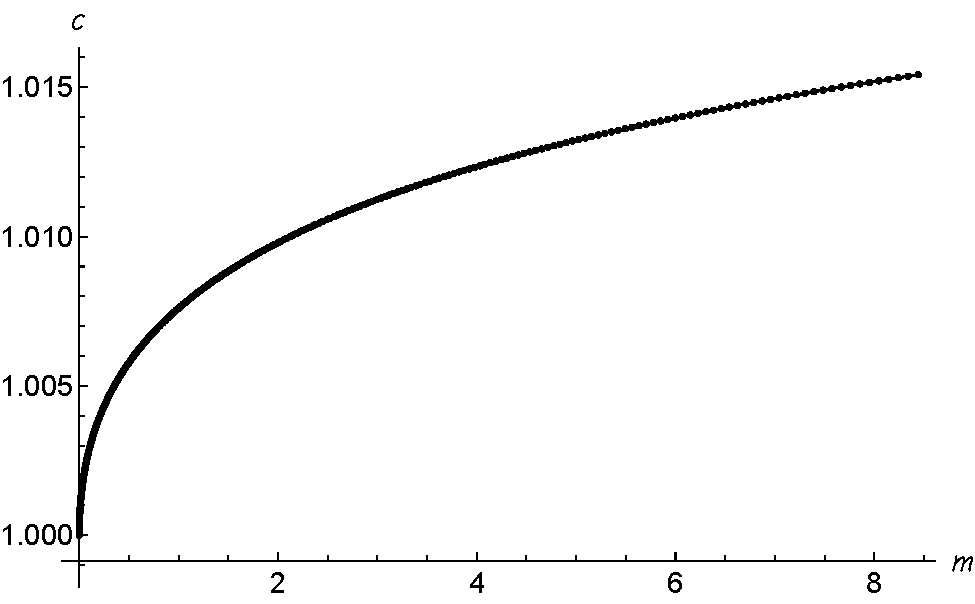
\includegraphics{\econtexRoot/\FigDirApndx/PFGICHoldsFHWCFailsRICFails}}
\caption{Nondegenerate Consumption Function with \cancel{FHWC} and \cancel{RIC}}
\label{fig:PFGICHoldsFHWCFailsRICFails}
\end{figure}

\begin{comment}
We can rewrite the expression for $\mathbb{C}$ from \eqref{PDVc} as:
\begin{eqnarray*}
   \mathbb{C}_{t-n}^{t} & = &  \left(\frac{\PatPGro^{-n}-\PatPGro^{-n}\PatR^{n+1}}{1-\PatR}\right)
\\ & = &  \left(\frac{\PatPGro^{-n}-\PatR\PGro^{n}/\Rfree^{n}}{1-\PatR}\right)
\\ & = &  \left(\frac{(\PGro/\Pat)^{n}-\PatR(\PGro/\Rfree)^{n}}{1-\PatR}\right)
\\ & = &  (\PGro/\Rfree)^{n}\left(\frac{(\Rfree/\Pat)^{n}-\PatR}{1-\PatR}\right)
\\ \Rnorm^{n}\mathbb{C}_{t-n}^{t}  & = &  \left(\frac{(\Rfree/\Pat)^{n}-\PatR}{1-\PatR}\right)
\end{eqnarray*}
but \cancel{RIC} implies that $\Pat > \Rfree$ so
\begin{eqnarray*}
\lim_{n \rightarrow \infty} \Rnorm^{n}\mathbb{C}_{t-n}^{t}  & = &  \left(\frac{-\PatR}{1-\PatR}\right)
\end{eqnarray*}
which means that in the limit
\begin{eqnarray}
\lim_{n \rightarrow \infty} \Rnorm^{n}\bRat_{\#}^{n} & = &  \left(\frac{-\PatR}{1-\PatR}\right) - \Rnorm^{n}\left(\frac{1-\Rnorm^{-1}\Rnorm^{-n}}{1-\Rnorm^{-1}}\right) %\label{eq:bPoundLim}
\\ & = & \left(\frac{-\PatR}{1-\PatR} + \frac{-\Rnorm^{-1}}{1-\Rnorm^{-1}}\right) - \left(\frac{\Rnorm^{n}}{1-\Rnorm^{-1}}\right)
\end{eqnarray}
so we can solve for the limiting $n$ as a function of $\bRat$ via
\begin{eqnarray}
  \bRat + \left(\frac{1}{1-\Rnorm^{-1}}\right) & = & \Rnorm^{-\hat{n}}\left(\frac{-\PatR}{1-\PatR} + \frac{-\Rnorm^{-1}}{1-\Rnorm^{-1}}\right)
\\ \log \left(\bRat + \left(\frac{1}{1-\Rnorm^{-1}}\right)\right) & = & -\hat{n} \log \Rnorm + \log \left(\frac{-\PatR}{1-\PatR} + \frac{-\Rnorm^{-1}}{1-\Rnorm^{-1}}\right)
\\ \frac{\log \left(\frac{-\PatR}{1-\PatR} + \frac{-\Rnorm^{-1}}{1-\Rnorm^{-1}}\right)-\log \left(\bRat + \left(\frac{1}{1-\Rnorm^{-1}}\right)\right)}{\log \Rnorm } & = & \hat{n}
\end{eqnarray}
which defines $\hat{\nFunc}(\bRat)$ which yields an approximation to the
value of $n$ associated with a given $\bRat$.

We can directly compute
\begin{eqnarray}
  \nabla & = & \bRat - \bRat_{\#}^{\hat{n}}
\end{eqnarray}
and can obtain a better appxoimation to the correct $n$ from
\begin{eqnarray}
  \hat{\hat{n}} & = &
\end{eqnarray}

We can obtain a more exact approximation to the correct ${n}$ by defining
\begin{eqnarray}
\nabla(n) \equiv   \lim_{n \rightarrow \infty}\Rnorm^{n}\mathbb{C}_{t-n}^{t}-\Rnorm^{n}\mathbb{C}_{t-n}^{t} & = &  \left(\frac{\PatR^{-n}}{1-\PatR}\right).
\end{eqnarray}
from which we can obtain the difference between the approximate and the exact $\mathbb{C}_{t-n}^{t}$ as $\Rnorm^{-n}\nabla(n)$ and


For this $n$ and
$\bRat$ we can obtain the corresponding
$\cRat=\PatPGro^{-\nFunc(\bRat)}$.  Note, however, that this is {\it not}
the level of $\cRat$ directly associated with $\bRat$ on the true
consumption function, because we used only a limiting approximation to
the correct $n$ rather than the correct $n$.

Our strategy, in this case, is

The limiting difference can be obtained by realizing that
\begin{eqnarray}
\nabla(n) \equiv   \lim_{n \rightarrow \infty}\Rnorm^{n}\mathbb{C}_{t-n}^{t}-\Rnorm^{n}\mathbb{C}_{t-n}^{t} & = &  \left(\frac{\PatR^{-n}}{1-\PatR}\right).
\end{eqnarray}
and so

\end{comment}

We can summarize as follows.  Given that the PF-GIC holds, the
interesting question is whether the FHWC holds.  If so, the
RIC automatically holds, and the solution limits
into the solution to the unconstrained problem as $\mRat \uparrow
\infty$.  But even if the FHWC fails, the problem has a
well-defined solution, whether or not the RIC holds.

%\end{verbatimwrite}\documentclass[../BufferStockTheory.tex]{subfiles}
\providecommand{\econtexRoot}{}
\renewcommand{\econtexRoot}{.}
 % Switch root to subdirectory 

\provideboolean{Metin}\setboolean{Metin}{true}\newcommand{\Metin}[2]{\ifthenelse{\boolean{Metin}}{\marginpar{\large Metin}\{{#1}\} $\rightarrow$ \{{#2}\}}{#2}}% PrivateMsg: Comments by Metin Uyanik

\begin{document}
\newcommand{\FigDirApndx}{Code/Mathematica/Results/BufferStockTheory/Figures}

%\begin{verbatimwrite}{\ApndxDir/ApndxSolnMethEndogGpts.tex}
\section{Perfect Foresight Liquidity Constrained Solution}\label{sec:ApndxLiqConstr}
%{\it Note: There is an inconsistency between the files ApndxLiqConstr.tex and ApndxLiqConstrStandAlone.tex files in the beginning of the first paragraph below. I accept ApndxLiqConstr.tex as valid and replace the first paragraph in this StandAlone version with the one in the output file. This seems counterintuitive since ApndxLiqConstr.tex is output of ApndxLiqConstrStandAlone.tex but the paragraph in the ApndxLiqConstr.tex file sounds better.} % MetinComment % PrivateMsg

  This appendix taxonomizes the characteristics of the limiting
  consumption function $\mathring{\cFunc}(\mRat)$ under perfect
  foresight in the presence of a liquidity constraint requiring $\bRat
  \geq 0$ under various conditions.  Results are summarized in
  table~\ref{table:LiqConstrScenarios}.

\newlength\LiqConstrScenariosWidth
\newsavebox{\LiqConstrScenarios}

\begin{table}[b]
\begin{center}
\caption{Taxonomy of Liquidity Constrained Model Outcomes}\label{table:LiqConstrScenarios}
\sbox{\LiqConstrScenarios}{
\begin{tabular}{|l|rcl|l|}\hline
Name & \multicolumn{3}{c|}{Condition}             & Outcome/Comments % & Example
\\ \hline
\cancel{PF-GIC}      & $\phantom{\Pat/\Rfree}$ & $\phantom{~<~}1        {~<~}$ & $        {\Pat/\PGro}$  & Constraint never binds for $\mRat \geq 1$ %& %$\{\Pat,\PGro\}=\{1,0.98\}$
\\ ~~~~RIC           & $        {\Pat/\Rfree}$ & $        {~<~}1\phantom{~<~}$ & $\phantom{\Pat/\PGro}$  & ~~FHWC holds ($\Rfree > \PGro$) % & $\{\Rfree,\Discount, \PGro \} = $
\\ ~~~~              &                         &                               &                         & ~~$\mathring{\cFunc}(\mRat) = \bar{\cFunc}(\mRat)$ for $\mRat \geq 1$ % & ~~$\{1.02,1.02^{-1},0.98\}$
\\ ~~~~\cancel{RIC}   & $\phantom{\Pat/\Rfree}$ & $\phantom{~<~}1        {~<~}$ & $        {\Pat/\Rfree}$ & ~~$\mathring{\cFunc}(\mRat)$ is degenerate %&
%\\ ~~~~               &                         &                               &                         &                                                            &
%\\ ~~~~~~\cancel{FHWC}& $        {\Rfree/\PGro}$ & $      {~<~}1        {~<~}$ & $        {\PGro/\Rfree}$ & $1 < \Pat/\Rfree < \Pat/\PGro$ & $\{\Rfree,\Discount, \PGro,\CRRA \} = $
%\\ ~~~~~~             &                          &                             &                          &                                & $~~\{0.98,1.00, 0.97,2 \} $
%\\ ~~~~~~        FHWC & $        {\PGro/\Rfree}$ & $      {~<~}1        {~<~}$ & $        {\Rfree/\PGro}$ & $1 < \Pat/\Rfree < \Pat/\PGro$ & $\{\Rfree,\Discount, \PGro,\CRRA \} = $
%\\ ~~~~~~             &                          &                             &                          &                                & $~~\{0.98,1.00, 0.97,2 \} $
\\ PF-GIC             & $        {\Pat/\PGro}$ & $        {~<~}1\phantom{~<~}$ & $\phantom{\Pat/\Rfree}$  & Constraint binds in finite time for any $\mRat$ % &
\\ ~~~~RIC            & $        {\Pat/\Rfree}$  & $      {~<~}1\phantom{~<~}$ & $\phantom{\Pat/\PGro}$   & ~~FHWC may or may not hold
\\ ~~~~               &                          &                             &                          & ~~$\lim_{m \uparrow \infty}\bar{\cFunc}(\mRat) - \mathring{\cFunc}(\mRat) = 0$ % & ~~$\{1.02,1.02^{-1},1.02\}$
\\ ~~~~               &                          &                             &                          & ~~$\lim_{m \uparrow \infty}\mathring{\MPCFunc}(\mRat) = \MinMPC$ % & ~~$\{1.02,1.02^{-1},1.02\}$
\\ ~~~~\cancel{RIC}   &                          & $\phantom{~<~}1         ~<~ $ & $         \Pat/\Rfree$ & ~~\cancel{FHWC}
\\ ~~~~~~             &                          &                             &                          &~~$\lim_{\mRat \uparrow \infty} \mathring{\MPCFunc}(\mRat) =  0$               % & ~~$\{0.98,1.00, 0.99, 2\} $
%\ ~~~~               &                          &                             &                          & ~~$\lim_{m \uparrow \infty}\bar{\cFunc}(\mRat) - \mathring{\cFunc}(\mRat) = 0$ % & ~~$\{1.02,1.02^{-1},1.02\}$
%\ ~~~~               &                          &                             &                          & ~~$\lim_{m \uparrow \infty}\mathring{\MPCFunc}(\mRat) = \MinMPC$ % & ~~$\{1.02,1.02^{-1},1.02\}$
%\ ~~~~FHWC           & $        {\PGro/\Rfree}$ & $      {~<~}1        {~<~}$ & $        {\Rfree/\PGro}$ & ~~RIC holds
%\ ~~~~\cancel{FHWC}  & $        {\Rfree/\PGro}$ & $      {~<~}1        {~<~}$ & $        {\PGro/\Rfree}$ & ~~$\mathring{\cFunc}(\mRat)$ nondegenerate % &
%\ ~~~~~~ RIC         & $        {\Pat/\Rfree} $ & $      {~<~}1\phantom{~<~}$ & $\phantom{\PGro/\Rfree}$ &~~~~$\lim_{m \uparrow \infty}\bar{\cFunc}(\mRat) - \mathring{\cFunc}(\mRat) = 0$ % & $\{\Rfree,\Discount, \PGro, \CRRA\}= $
%\ ~~~~~~             &                          &                             &                          &~~~~$\lim_{\mRat \uparrow \infty} \mathring{\MPCFunc}(\mRat) =  \MinMPC$ % & ~~$\{1.02,1.02^{-1},1.03,2\} $
%\ ~~~~~~ \cancel{RIC}& $\phantom{\Pat/\Rfree} $ & $\phantom{~<~}1      {~<~}$ & $        {\Pat/\Rfree}$  &~~~~$\lim_{\mRat \uparrow \infty} \mathring{\MPCFunc}(\mRat) =  0$               % & ~~$\{0.98,1.00, 0.99, 2\} $
\\ \hline
\end{tabular}
} % End \sbox

\settowidth\LiqConstrScenariosWidth{\usebox{\LiqConstrScenarios}}
\usebox{\LiqConstrScenarios}
\parbox{\LiqConstrScenariosWidth}{\footnotesize Conditions are applied from left to right; for example, the second and third rows indicate conclusions in the case where \cancel{PF-GIC} and RIC both hold, while the fourth row indicates that when the PF-GIC and the RIC both fail, the consumption function is degenerate; the next row indicates that whenever the PF-GIC holds, the constraint will bind in finite time.}

\medskip
\end{center}
\end{table}




\subsection{If PF-GIC Fails}

A consumer is `growth patient' if the perfect foresight growth
impatience condition fails (\cancel{PF-GIC}, $1 < \Pat/\PGro$).  Under
\cancel{PF-GIC} the constraint does not bind at the lowest feasible value of $\mRat_{t}=1$ because
$1 < (\Rfree\Discount)^{1/\CRRA}/\PGro$ implies that spending
everything today (setting $\cRat_{t}=\mRat_{t}=1$) produces lower
marginal utility than is obtainable by reallocating a marginal unit of
resources to the next period at return $\Rfree$:\footnote{The point at
  which the constraint would bind (if that point could be attained) is
  the $\mRat=\cRat$ for which $\util^{\prime}(\cRat_{\#}) = \Rfree
  \Discount \util^{\prime}(\PGro)$ which is $\cRat_{\#} =
  \PGro/(\Rfree \Discount)^{1/\CRRA}$ and the consumption function
  will be defined by
  $\mathring{\cFunc}(\mRat)=\min[\mRat,\cRat_{\#}+(\mRat-\cRat_{\#})\MinMPC
  ]$.}
\begin{eqnarray}
1 & < & (\Rfree \Discount)^{1/\CRRA}\PGro^{-1}   \label{eq:EulerPFGICFails}
\\ 1 & < & \Rfree \Discount \PGro^{-\CRRA}
\\  \util^{\prime}(1) & < & \Rfree \Discount \util^{\prime}(\PGro)   \label{eq:EulerPFGICFailsEnd}.
\end{eqnarray}

Similar logic shows that under these circumstances the constraint will
never bind for a constrained consumer with a finite horizon of $n$
periods, so such a consumer's consumption function will be the same as for the
unconstrained case examined in the main text.

If the RIC fails ($1 < \PatR$) while the finite human wealth condition
holds, the limiting value of this consumption function as $n \uparrow
\infty$ is the degenerate function
\begin{eqnarray}
  \mathring{\cFunc}_{T-n}(\mRat) & = & 0 (\bRat_{t}+\hRat).
\end{eqnarray}

If the RIC fails and the FHWC fails, human wealth limits to $\hRat =
\infty$ so the consumption function limits to either
$\mathring{\cFunc}_{T-n}(\mRat) = 0$ or
$\mathring{\cFunc}_{T-n}(\mRat) = \infty$ depending on the relative
speeds with which the MPC approaches zero and human wealth approaches
$\infty$.\footnote{The knife-edge case is where $\Pat = \PGro$, in
  which case the two quantites counterbalance and the limiting
  function is $\mathring{\cFunc}(\mRat)=\min[\mRat,1]$.}

Thus, the requirement that the consumption function be nondegenerate
implies that for a consumer satisfying \cancel{PF-GIC} we must impose
the RIC (and the FHWC can be shown to be a consequence of \cancel{PF-GIC} and RIC).  In
this case, the consumer's optimal behavior is easy to describe.  We
can calculate the point at which the unconstrained consumer would
choose $\cRat = \mRat$ from \eqref{eq:cFuncPFUnc}:
\begin{eqnarray}
  \mRat_{\#} & = & (\mRat_{\#}-1+\hRat)\MinMPC
\\ \mRat_{\#}(1-\MinMPC) & = & (\hRat - 1)\MinMPC
\\ \mRat_{\#} & = & (\hRat - 1)\left(\frac{\MinMPC}{1-\MinMPC}\right)
\end{eqnarray}
which (under these assumptions) satisfies $0 < \mRat_{\#} < 1$.\footnote{Note that $0 < \mRat_{\#}$ is implied by RIC and $ \mRat_{\#}<1$ is implied by \mbox{\cancel{PF-GIC}}.}  For
$\mRat < \mRat_{\#}$ the unconstrained consumer would choose to
consume more than $\mRat$; for such $\mRat$, the constrained consumer
is obliged to choose $\mathring{\cFunc}(\mRat) = \mRat$.\footnote{As an
  illustration, consider a consumer for whom $\Pat = 1$, $\Rfree
  =1.01$ and $\PGro = 0.99$.  This consumer will save the amount
  necessary to ensure that growth in market wealth exactly offsets the
  decline in human wealth represented by $\PGro < 1$; total wealth
  (and therefore total consumption) will remain constant, even as
  market wealth and human wealth trend in opposite directions.}  For
any $\mRat > \mRat_{\#}$ the constraint will never bind and the
consumer will choose to spend the same amount as the unconstrained
consumer, $\bar{\cFunc}(\mRat)$.


\subsection{If PF-GIC Holds}

Imposition of the PF-GIC reverses the inequality in
\eqref{eq:EulerPFGICFails}-\eqref{eq:EulerPFGICFailsEnd}, and thus
reverses the conclusion: A consumer who starts with $\mRat_{t}=1$ will
desire to consume more than 1.  Such a consumer will be constrained,
not only in period $t$, but perpetually thereafter.

Now define $\bRat_{\#}^{n}$ as the $\bRat_{t}$ such that
an unconstrained consumer holding $\bRat_{t}=\bRat_{\#}^{n}$ would behave so as to arrive in period $t+n$ with $\bRat_{t+n}=0$ (with $\bRat_{\#}^{0}$ trivially equal to 0); for example, a consumer with $\bRat_{t-1}=\bRat_{\#}^{1}$ was on the `cusp' of being constrained in period
$t-1$: Had $b_{t-1}$ been infinitesimally smaller, the constraint
would have been binding (because the consumer would have desired, but
been unable, to enter period $t$ with negative, not zero, $b$).  Given
the PF-GIC, the constraint certainly binds in period $t$ (and
thereafter) with resources of
$\mRat_{t}=\mRat_{\#}^{0}=1+\bRat_{\#}^{0}=1$: The consumer cannot
spend more (because constrained), and will not choose to spend less
(because impatient), than $c_{t}=\cRat_{\#}^{0}=1$.

We can construct the entire `prehistory' of this consumer leading up to $t$ as follows.
Maintaining the assumption that the constraint has never bound in the past,
$\cRat$ must have been growing according to $\PatPGro$, so consumption $n$ periods in the past must have been
\begin{eqnarray}
  \cRat_{\#}^{n} & = & \PatPGro^{-n} \cRat_{t} = \PatPGro^{-n}. \label{eq:cPreHist}
\end{eqnarray}

The PDV of consumption from $t-n$ until $t$ can thus be computed as
\begin{eqnarray}
   \mathbb{C}_{t-n}^{t} & = & \cRat_{t-n}(1+\Pat/\Rfree+ ... + (\Pat/\Rfree)^{n}) \notag
% \\   \mathbb{C}_{t-n}^{t} & = & \cRat_{t-n}(1+\PatPGro/\Rnorm+ ... + (\PatPGro/\Rnorm)^{n}) \notag
\\ & = & \cRat_{\#}^{n}(1+\PatR+ ... + \PatR^{n}) \notag
\\ & = & \PatPGro^{-n}\left(\frac{1-\PatR^{n+1}}{1-\PatR}\right) \label{PDVc}
\end{eqnarray}
and note that the consumer's human wealth between $t-n$ and $t$ (the relevant
time horizon, because from $t$ onward the consumer will be constrained
and unable to access post-$t$ income) is
\begin{eqnarray}
  \hRat_{\#}^{n} & = & 1+...+\Rnorm^{-n}
\end{eqnarray}
while the intertemporal budget constraint says
\begin{eqnarray*}
  \mathbb{C}_{t-n}^{t} & = & \bRat_{\#}^{n}+\hRat_{\#}^{n}
\end{eqnarray*}
from which we can solve for the $\bRat_{\#}^{n}$ such that
the consumer with $\bRat_{t-n} = \bRat_{\#}^{n}$ would
unconstrainedly plan (in period $t-n$) to arrive in period $t$ with
$\bRat_{t}=0$:
\begin{eqnarray}
\bRat_{\#}^{n} & =&  \mathbb{C}_{t-n}^{t} - \overbrace{\left(\frac{1-\Rnorm^{-(n+1)}}{1-\Rnorm^{-1}}\right)}^{\hRat_{\#}^{n}} \label{eq:bPound}.
\end{eqnarray}

Defining $\mRat_{\#}^{n}=\bRat_{\#}^{n}+1$, consider the function
$\mathring{\cFunc}(\mRat)$ defined by linearly connecting the points
$\{\mRat_{\#}^{n},\cRat_{\#}^{n}\}$ for integer values of $n \geq 0$
(and setting $\mathring{\cFunc}(\mRat)=\mRat$ for $\mRat<1$).  This
function will return, for any value of $\mRat$, the optimal value of
$\cRat$ for a liquidity constrained consumer with an infinite horizon.
The function is piecewise linear with `kink points' where the slope
discretely changes, because for infinitesimal $\epsilon$ the MPC of a
consumer with assets $\mRat=\mRat_{\#}^{n}-\epsilon$ is discretely
higher than for a consumer with assets $\mRat=\mRat_{\#}^{n}+\epsilon$
because the latter consumer will spread a marginal dollar over more
periods before exhausting it.

In order for a unique consumption function to be defined by this
sequence \eqref{eq:bPound} for the entire domain of positive real
values of $b$, we need $\bRat_{\#}^{n}$ to become arbitrarily large with
$n$.  That is, we need
\begin{eqnarray}
  \lim_{n \rightarrow \infty} \bRat_{\#}^{n} = \infty. \label{eq:bToInfty}
\end{eqnarray}

\subsubsection{If FHWC Holds}
The FHWC requires $\Rnorm^{-1} < 1$, in which case the second term in \eqref{eq:bPound} limits to a constant as $n \uparrow \infty$, and \eqref{eq:bToInfty} reduces to a requirement that
\begin{eqnarray*}
  \lim_{n \rightarrow \infty} \left(\frac{\PatPGro^{-n}-(\PatR/\PatPGro)^{n}\PatR}{1-\PatR}\right) & = & \infty
\\  \lim_{n \rightarrow \infty} \left(\frac{\PatPGro^{-n}-\Rnorm^{-n}\PatR}{1-\PatR}\right) & = & \infty
\\  \lim_{n \rightarrow \infty} \left(\frac{\PatPGro^{-n}}{1-\PatR}\right) & = & \infty.
\end{eqnarray*}
Given the PF-GIC $\PatPGro^{-1}>1$, this will hold iff the RIC holds, $\PatR < 1$.  But given that the FHWC
$\Rfree > \PGro$ holds, the PF-GIC is stronger (harder to satisfy) than the RIC; thus, FHWC
and the PF-GIC together imply the RIC, and so a well-defined
solution exists.  Furthermore, in the limit as $n$ approaches
infinity, the difference between the limiting constrained consumption
function and the unconstrained consumption function becomes
vanishingly small, because as the date at which the constraint binds
becomes arbitrarily distant, the effect of that constraint on current
behavior shrinks to nothing.  That is,
\begin{eqnarray}
\lim_{m \rightarrow \infty}\mathring{\cFunc}(m) - \bar{\cFunc}(m) = 0.
\end{eqnarray}

% Finally, the main text shows that the PF-GIC is a stronger condition than the PF-FVR; that is, PF-GIC $\Rightarrow$ PF-FVR.

\subsubsection{If FHWC Fails}
If the FHWC fails, matters are a bit more complex.
\begin{comment}
As noted in the main text, the Finite Value Requirement for such a consumer
requires $\PatPGro < (\Rfree/\PGro)^{1/\CRRA}$,\footnote{A
  unique well-defined nondegenerate limiting consumption function can
  actually exist even if a nondegenerate value function does not.  But
  the parametric combinations required for this are somewhat peculiar
  (including both $\Rfree < 1$ and $\PGro < 1$); but we restrict our attention
  to the more useful and plausible cases with finite value.} which is stronger (holds
in strictly fewer circumstances) than the PF-GIC condition $\PatPGro < 1$.
Thus, the PF-GIC is an implication of \cancel{FHWC}.
\end{comment}
Given failure of FHWC, \eqref{eq:bToInfty} requires

\begin{eqnarray}
%  \lim_{n \rightarrow \infty} \left(\frac{\PatPGro^{-n}-\Rnorm^{-n}\PatR}{1-\PatR}\right) + \left(\frac{1-\Rnorm^{-(n+1)}}{\Rnorm^{-1}-1}\right) & = & \infty \\
  \lim_{n \rightarrow \infty} \left(\frac{\Rnorm^{-n}\PatR-\PatPGro^{-n}}{\PatR-1}\right) + \left(\frac{1-\Rnorm^{-(n+1)}}{\Rnorm^{-1}-1}\right) & = & \infty \notag
\\   \lim_{n \rightarrow \infty} \left(\frac{\PatR}{\PatR-1}-\frac{\Rnorm^{-1}}{\Rnorm^{-1}-1}\right)\Rnorm^{-n}-\left(\frac{\PatPGro^{-n}}{\PatR-1}\right) & = & \infty \notag
\\   \lim_{n \rightarrow \infty} \left(\frac{\PatR(\Rnorm^{-1}-1)}{(\Rnorm^{-1}-1)(\PatR-1)}-\frac{\Rnorm^{-1}(\PatR-1)}{(\Rnorm^{-1}-1)(\PatR-1)}\right)\Rnorm^{-n}-\left(\frac{\PatPGro^{-n}}{\PatR-1}\right) & = & \infty. \label{eq:FHWCfails}
\end{eqnarray}

{\bf If RIC Holds}.  When the RIC holds, rearranging \eqref{eq:FHWCfails} gives
\begin{eqnarray*}
  \lim_{n \rightarrow \infty} \left(\frac{\PatPGro^{-n}}{1-\PatR}\right)-\Rnorm^{-n}\left(\frac{\PatR}{1-\PatR}+\frac{\Rnorm^{-1}}{\Rnorm^{-1}-1}\right) & = & \infty
\end{eqnarray*}
and for this to be true we need
\begin{eqnarray*}
  \PatPGro^{-1} & > & \Rnorm^{-1}
\\ \PGro/\Pat & > & \PGro/\Rfree
\\ 1 & > & \Pat/\Rfree
\end{eqnarray*}
which is merely the RIC again.  So the problem has a solution if the RIC holds.  Indeed,
we can even calculate the limiting MPC from
\begin{eqnarray}
  \lim_{n \rightarrow \infty} \MPC^{n}_{\#} & = & \lim_{n \rightarrow \infty} \left(\frac{\cRat_{\#}^{n}}{\bRat_{\#}^{n}}\right)
\end{eqnarray}
which with a few lines of algebra
\begin{comment}
Calculate the limit of
\begin{eqnarray}
\left(\frac{\PatPGro^{-n}}{\PatPGro^{-n}/(1-\PatR) - (1-\Rnorm^{-1}\Rnorm^{-n})/(1-\Rnorm^{-1})}\right) & = & \left(\frac{1}{1/(1-\PatR) + \Rnorm^{-n}\Rnorm^{-1}/(1-\Rnorm^{-1})}\right)
\end{eqnarray}
\end{comment}
can be shown to asymptote to the MPC in the perfect foresight model:\footnote{For an example of this configuration of parameters, see the notebook \texttt{doApndxLiqConstr.nb} in the software archive.}
\begin{eqnarray}
  \lim_{m \rightarrow \infty} \mathring{\pmb{\MPC}}(\mRat) & = & 1-\PatR.
\end{eqnarray}

{\bf If RIC Fails}.  Consider now the \cancel{RIC} case, $\PatR > 1$.  In this case the constant multiplying
$\Rnorm^{-n}$ in \eqref{eq:FHWCfails} will be positive if
\begin{eqnarray*}
  \PatR \Rnorm^{-1} - \PatR & > &  \Rnorm^{-1}\PatR-\Rnorm^{-1}
\\ \Rnorm^{-1} & > & \PatR
\\ \PGro & > & \Pat
\end{eqnarray*}
which is merely the PF-GIC which we are maintaining.  So the first term's limit is $+\infty$.  The
combined limit will be $+\infty$ if the term involving $\Rnorm^{-n}$
goes to $+\infty$ faster than the term involving $-\PatPGro^{-n}$ goes to
$-\infty$; that is, if
\begin{eqnarray*}
  \Rnorm^{-1} & > & \PatPGro^{-1}
\\ \PGro/\Rfree & > & \PGro/\Pat
\\ \Pat/\Rfree & > & 1
\end{eqnarray*}
which merely confirms the starting assumption that the RIC fails.
Thus, surprisingly, the problem has a well defined solution with
infinite human wealth if the RIC fails.  It remains true that \cancel{RIC}
implies a limiting MPC of zero,
\begin{eqnarray}
  \lim_{\mRat \rightarrow \infty} \mathring{\pmb{\MPC}}(\mRat)  & = & 0,
\end{eqnarray}
but that limit is approached gradually, starting from a positive
value, and consequently the consumption function is {\it not} the
degenerate $\mathring{\cFunc}(\mRat)=0$.  (Figure~\ref{fig:PFGICHoldsFHWCFailsRICFails} presents an example for $\CRRA=2$, $\Rfree=0.98$, $\Discount = 0.99$, $\PGro = 1.0$).

\begin{figure}
\centerline{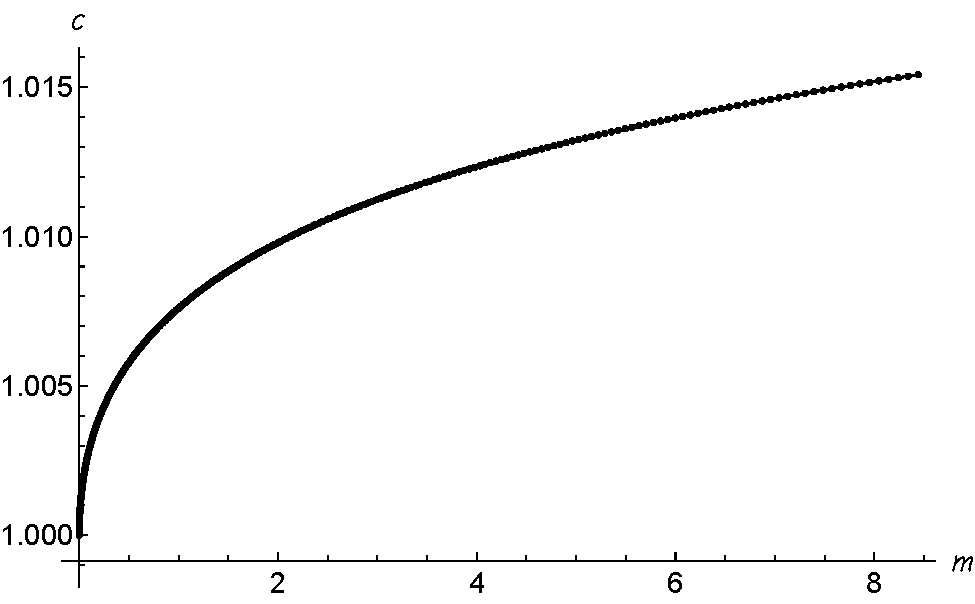
\includegraphics{\econtexRoot/\FigDirApndx/PFGICHoldsFHWCFailsRICFails}}
\caption{Nondegenerate Consumption Function with \cancel{FHWC} and \cancel{RIC}}
\label{fig:PFGICHoldsFHWCFailsRICFails}
\end{figure}

\begin{comment}
We can rewrite the expression for $\mathbb{C}$ from \eqref{PDVc} as:
\begin{eqnarray*}
   \mathbb{C}_{t-n}^{t} & = &  \left(\frac{\PatPGro^{-n}-\PatPGro^{-n}\PatR^{n+1}}{1-\PatR}\right)
\\ & = &  \left(\frac{\PatPGro^{-n}-\PatR\PGro^{n}/\Rfree^{n}}{1-\PatR}\right)
\\ & = &  \left(\frac{(\PGro/\Pat)^{n}-\PatR(\PGro/\Rfree)^{n}}{1-\PatR}\right)
\\ & = &  (\PGro/\Rfree)^{n}\left(\frac{(\Rfree/\Pat)^{n}-\PatR}{1-\PatR}\right)
\\ \Rnorm^{n}\mathbb{C}_{t-n}^{t}  & = &  \left(\frac{(\Rfree/\Pat)^{n}-\PatR}{1-\PatR}\right)
\end{eqnarray*}
but \cancel{RIC} implies that $\Pat > \Rfree$ so
\begin{eqnarray*}
\lim_{n \rightarrow \infty} \Rnorm^{n}\mathbb{C}_{t-n}^{t}  & = &  \left(\frac{-\PatR}{1-\PatR}\right)
\end{eqnarray*}
which means that in the limit
\begin{eqnarray}
\lim_{n \rightarrow \infty} \Rnorm^{n}\bRat_{\#}^{n} & = &  \left(\frac{-\PatR}{1-\PatR}\right) - \Rnorm^{n}\left(\frac{1-\Rnorm^{-1}\Rnorm^{-n}}{1-\Rnorm^{-1}}\right) %\label{eq:bPoundLim}
\\ & = & \left(\frac{-\PatR}{1-\PatR} + \frac{-\Rnorm^{-1}}{1-\Rnorm^{-1}}\right) - \left(\frac{\Rnorm^{n}}{1-\Rnorm^{-1}}\right)
\end{eqnarray}
so we can solve for the limiting $n$ as a function of $\bRat$ via
\begin{eqnarray}
  \bRat + \left(\frac{1}{1-\Rnorm^{-1}}\right) & = & \Rnorm^{-\hat{n}}\left(\frac{-\PatR}{1-\PatR} + \frac{-\Rnorm^{-1}}{1-\Rnorm^{-1}}\right)
\\ \log \left(\bRat + \left(\frac{1}{1-\Rnorm^{-1}}\right)\right) & = & -\hat{n} \log \Rnorm + \log \left(\frac{-\PatR}{1-\PatR} + \frac{-\Rnorm^{-1}}{1-\Rnorm^{-1}}\right)
\\ \frac{\log \left(\frac{-\PatR}{1-\PatR} + \frac{-\Rnorm^{-1}}{1-\Rnorm^{-1}}\right)-\log \left(\bRat + \left(\frac{1}{1-\Rnorm^{-1}}\right)\right)}{\log \Rnorm } & = & \hat{n}
\end{eqnarray}
which defines $\hat{\nFunc}(\bRat)$ which yields an approximation to the
value of $n$ associated with a given $\bRat$.

We can directly compute
\begin{eqnarray}
  \nabla & = & \bRat - \bRat_{\#}^{\hat{n}}
\end{eqnarray}
and can obtain a better appxoimation to the correct $n$ from
\begin{eqnarray}
  \hat{\hat{n}} & = &
\end{eqnarray}

We can obtain a more exact approximation to the correct ${n}$ by defining
\begin{eqnarray}
\nabla(n) \equiv   \lim_{n \rightarrow \infty}\Rnorm^{n}\mathbb{C}_{t-n}^{t}-\Rnorm^{n}\mathbb{C}_{t-n}^{t} & = &  \left(\frac{\PatR^{-n}}{1-\PatR}\right).
\end{eqnarray}
from which we can obtain the difference between the approximate and the exact $\mathbb{C}_{t-n}^{t}$ as $\Rnorm^{-n}\nabla(n)$ and


For this $n$ and
$\bRat$ we can obtain the corresponding
$\cRat=\PatPGro^{-\nFunc(\bRat)}$.  Note, however, that this is {\it not}
the level of $\cRat$ directly associated with $\bRat$ on the true
consumption function, because we used only a limiting approximation to
the correct $n$ rather than the correct $n$.

Our strategy, in this case, is

The limiting difference can be obtained by realizing that
\begin{eqnarray}
\nabla(n) \equiv   \lim_{n \rightarrow \infty}\Rnorm^{n}\mathbb{C}_{t-n}^{t}-\Rnorm^{n}\mathbb{C}_{t-n}^{t} & = &  \left(\frac{\PatR^{-n}}{1-\PatR}\right).
\end{eqnarray}
and so

\end{comment}

We can summarize as follows.  Given that the PF-GIC holds, the
interesting question is whether the FHWC holds.  If so, the
RIC automatically holds, and the solution limits
into the solution to the unconstrained problem as $\mRat \uparrow
\infty$.  But even if the FHWC fails, the problem has a
well-defined solution, whether or not the RIC holds.

%\end{verbatimwrite}\documentclass[../BufferStockTheory.tex]{subfiles}
\providecommand{\econtexRoot}{}
\renewcommand{\econtexRoot}{.}
 % Switch root to subdirectory 

\provideboolean{Metin}\setboolean{Metin}{true}\newcommand{\Metin}[2]{\ifthenelse{\boolean{Metin}}{\marginpar{\large Metin}\{{#1}\} $\rightarrow$ \{{#2}\}}{#2}}% PrivateMsg: Comments by Metin Uyanik

\begin{document}
\newcommand{\FigDirApndx}{Code/Mathematica/Results/BufferStockTheory/Figures}

%\begin{verbatimwrite}{\ApndxDir/ApndxSolnMethEndogGpts.tex}
\section{Perfect Foresight Liquidity Constrained Solution}\label{sec:ApndxLiqConstr}
%{\it Note: There is an inconsistency between the files ApndxLiqConstr.tex and ApndxLiqConstrStandAlone.tex files in the beginning of the first paragraph below. I accept ApndxLiqConstr.tex as valid and replace the first paragraph in this StandAlone version with the one in the output file. This seems counterintuitive since ApndxLiqConstr.tex is output of ApndxLiqConstrStandAlone.tex but the paragraph in the ApndxLiqConstr.tex file sounds better.} % MetinComment % PrivateMsg

  This appendix taxonomizes the characteristics of the limiting
  consumption function $\mathring{\cFunc}(\mRat)$ under perfect
  foresight in the presence of a liquidity constraint requiring $\bRat
  \geq 0$ under various conditions.  Results are summarized in
  table~\ref{table:LiqConstrScenarios}.

\newlength\LiqConstrScenariosWidth
\newsavebox{\LiqConstrScenarios}

\begin{table}[b]
\begin{center}
\caption{Taxonomy of Liquidity Constrained Model Outcomes}\label{table:LiqConstrScenarios}
\sbox{\LiqConstrScenarios}{
\begin{tabular}{|l|rcl|l|}\hline
Name & \multicolumn{3}{c|}{Condition}             & Outcome/Comments % & Example
\\ \hline
\cancel{PF-GIC}      & $\phantom{\Pat/\Rfree}$ & $\phantom{~<~}1        {~<~}$ & $        {\Pat/\PGro}$  & Constraint never binds for $\mRat \geq 1$ %& %$\{\Pat,\PGro\}=\{1,0.98\}$
\\ ~~~~RIC           & $        {\Pat/\Rfree}$ & $        {~<~}1\phantom{~<~}$ & $\phantom{\Pat/\PGro}$  & ~~FHWC holds ($\Rfree > \PGro$) % & $\{\Rfree,\Discount, \PGro \} = $
\\ ~~~~              &                         &                               &                         & ~~$\mathring{\cFunc}(\mRat) = \bar{\cFunc}(\mRat)$ for $\mRat \geq 1$ % & ~~$\{1.02,1.02^{-1},0.98\}$
\\ ~~~~\cancel{RIC}   & $\phantom{\Pat/\Rfree}$ & $\phantom{~<~}1        {~<~}$ & $        {\Pat/\Rfree}$ & ~~$\mathring{\cFunc}(\mRat)$ is degenerate %&
%\\ ~~~~               &                         &                               &                         &                                                            &
%\\ ~~~~~~\cancel{FHWC}& $        {\Rfree/\PGro}$ & $      {~<~}1        {~<~}$ & $        {\PGro/\Rfree}$ & $1 < \Pat/\Rfree < \Pat/\PGro$ & $\{\Rfree,\Discount, \PGro,\CRRA \} = $
%\\ ~~~~~~             &                          &                             &                          &                                & $~~\{0.98,1.00, 0.97,2 \} $
%\\ ~~~~~~        FHWC & $        {\PGro/\Rfree}$ & $      {~<~}1        {~<~}$ & $        {\Rfree/\PGro}$ & $1 < \Pat/\Rfree < \Pat/\PGro$ & $\{\Rfree,\Discount, \PGro,\CRRA \} = $
%\\ ~~~~~~             &                          &                             &                          &                                & $~~\{0.98,1.00, 0.97,2 \} $
\\ PF-GIC             & $        {\Pat/\PGro}$ & $        {~<~}1\phantom{~<~}$ & $\phantom{\Pat/\Rfree}$  & Constraint binds in finite time for any $\mRat$ % &
\\ ~~~~RIC            & $        {\Pat/\Rfree}$  & $      {~<~}1\phantom{~<~}$ & $\phantom{\Pat/\PGro}$   & ~~FHWC may or may not hold
\\ ~~~~               &                          &                             &                          & ~~$\lim_{m \uparrow \infty}\bar{\cFunc}(\mRat) - \mathring{\cFunc}(\mRat) = 0$ % & ~~$\{1.02,1.02^{-1},1.02\}$
\\ ~~~~               &                          &                             &                          & ~~$\lim_{m \uparrow \infty}\mathring{\MPCFunc}(\mRat) = \MinMPC$ % & ~~$\{1.02,1.02^{-1},1.02\}$
\\ ~~~~\cancel{RIC}   &                          & $\phantom{~<~}1         ~<~ $ & $         \Pat/\Rfree$ & ~~\cancel{FHWC}
\\ ~~~~~~             &                          &                             &                          &~~$\lim_{\mRat \uparrow \infty} \mathring{\MPCFunc}(\mRat) =  0$               % & ~~$\{0.98,1.00, 0.99, 2\} $
%\ ~~~~               &                          &                             &                          & ~~$\lim_{m \uparrow \infty}\bar{\cFunc}(\mRat) - \mathring{\cFunc}(\mRat) = 0$ % & ~~$\{1.02,1.02^{-1},1.02\}$
%\ ~~~~               &                          &                             &                          & ~~$\lim_{m \uparrow \infty}\mathring{\MPCFunc}(\mRat) = \MinMPC$ % & ~~$\{1.02,1.02^{-1},1.02\}$
%\ ~~~~FHWC           & $        {\PGro/\Rfree}$ & $      {~<~}1        {~<~}$ & $        {\Rfree/\PGro}$ & ~~RIC holds
%\ ~~~~\cancel{FHWC}  & $        {\Rfree/\PGro}$ & $      {~<~}1        {~<~}$ & $        {\PGro/\Rfree}$ & ~~$\mathring{\cFunc}(\mRat)$ nondegenerate % &
%\ ~~~~~~ RIC         & $        {\Pat/\Rfree} $ & $      {~<~}1\phantom{~<~}$ & $\phantom{\PGro/\Rfree}$ &~~~~$\lim_{m \uparrow \infty}\bar{\cFunc}(\mRat) - \mathring{\cFunc}(\mRat) = 0$ % & $\{\Rfree,\Discount, \PGro, \CRRA\}= $
%\ ~~~~~~             &                          &                             &                          &~~~~$\lim_{\mRat \uparrow \infty} \mathring{\MPCFunc}(\mRat) =  \MinMPC$ % & ~~$\{1.02,1.02^{-1},1.03,2\} $
%\ ~~~~~~ \cancel{RIC}& $\phantom{\Pat/\Rfree} $ & $\phantom{~<~}1      {~<~}$ & $        {\Pat/\Rfree}$  &~~~~$\lim_{\mRat \uparrow \infty} \mathring{\MPCFunc}(\mRat) =  0$               % & ~~$\{0.98,1.00, 0.99, 2\} $
\\ \hline
\end{tabular}
} % End \sbox

\settowidth\LiqConstrScenariosWidth{\usebox{\LiqConstrScenarios}}
\usebox{\LiqConstrScenarios}
\parbox{\LiqConstrScenariosWidth}{\footnotesize Conditions are applied from left to right; for example, the second and third rows indicate conclusions in the case where \cancel{PF-GIC} and RIC both hold, while the fourth row indicates that when the PF-GIC and the RIC both fail, the consumption function is degenerate; the next row indicates that whenever the PF-GIC holds, the constraint will bind in finite time.}

\medskip
\end{center}
\end{table}




\subsection{If PF-GIC Fails}

A consumer is `growth patient' if the perfect foresight growth
impatience condition fails (\cancel{PF-GIC}, $1 < \Pat/\PGro$).  Under
\cancel{PF-GIC} the constraint does not bind at the lowest feasible value of $\mRat_{t}=1$ because
$1 < (\Rfree\Discount)^{1/\CRRA}/\PGro$ implies that spending
everything today (setting $\cRat_{t}=\mRat_{t}=1$) produces lower
marginal utility than is obtainable by reallocating a marginal unit of
resources to the next period at return $\Rfree$:\footnote{The point at
  which the constraint would bind (if that point could be attained) is
  the $\mRat=\cRat$ for which $\util^{\prime}(\cRat_{\#}) = \Rfree
  \Discount \util^{\prime}(\PGro)$ which is $\cRat_{\#} =
  \PGro/(\Rfree \Discount)^{1/\CRRA}$ and the consumption function
  will be defined by
  $\mathring{\cFunc}(\mRat)=\min[\mRat,\cRat_{\#}+(\mRat-\cRat_{\#})\MinMPC
  ]$.}
\begin{eqnarray}
1 & < & (\Rfree \Discount)^{1/\CRRA}\PGro^{-1}   \label{eq:EulerPFGICFails}
\\ 1 & < & \Rfree \Discount \PGro^{-\CRRA}
\\  \util^{\prime}(1) & < & \Rfree \Discount \util^{\prime}(\PGro)   \label{eq:EulerPFGICFailsEnd}.
\end{eqnarray}

Similar logic shows that under these circumstances the constraint will
never bind for a constrained consumer with a finite horizon of $n$
periods, so such a consumer's consumption function will be the same as for the
unconstrained case examined in the main text.

If the RIC fails ($1 < \PatR$) while the finite human wealth condition
holds, the limiting value of this consumption function as $n \uparrow
\infty$ is the degenerate function
\begin{eqnarray}
  \mathring{\cFunc}_{T-n}(\mRat) & = & 0 (\bRat_{t}+\hRat).
\end{eqnarray}

If the RIC fails and the FHWC fails, human wealth limits to $\hRat =
\infty$ so the consumption function limits to either
$\mathring{\cFunc}_{T-n}(\mRat) = 0$ or
$\mathring{\cFunc}_{T-n}(\mRat) = \infty$ depending on the relative
speeds with which the MPC approaches zero and human wealth approaches
$\infty$.\footnote{The knife-edge case is where $\Pat = \PGro$, in
  which case the two quantites counterbalance and the limiting
  function is $\mathring{\cFunc}(\mRat)=\min[\mRat,1]$.}

Thus, the requirement that the consumption function be nondegenerate
implies that for a consumer satisfying \cancel{PF-GIC} we must impose
the RIC (and the FHWC can be shown to be a consequence of \cancel{PF-GIC} and RIC).  In
this case, the consumer's optimal behavior is easy to describe.  We
can calculate the point at which the unconstrained consumer would
choose $\cRat = \mRat$ from \eqref{eq:cFuncPFUnc}:
\begin{eqnarray}
  \mRat_{\#} & = & (\mRat_{\#}-1+\hRat)\MinMPC
\\ \mRat_{\#}(1-\MinMPC) & = & (\hRat - 1)\MinMPC
\\ \mRat_{\#} & = & (\hRat - 1)\left(\frac{\MinMPC}{1-\MinMPC}\right)
\end{eqnarray}
which (under these assumptions) satisfies $0 < \mRat_{\#} < 1$.\footnote{Note that $0 < \mRat_{\#}$ is implied by RIC and $ \mRat_{\#}<1$ is implied by \mbox{\cancel{PF-GIC}}.}  For
$\mRat < \mRat_{\#}$ the unconstrained consumer would choose to
consume more than $\mRat$; for such $\mRat$, the constrained consumer
is obliged to choose $\mathring{\cFunc}(\mRat) = \mRat$.\footnote{As an
  illustration, consider a consumer for whom $\Pat = 1$, $\Rfree
  =1.01$ and $\PGro = 0.99$.  This consumer will save the amount
  necessary to ensure that growth in market wealth exactly offsets the
  decline in human wealth represented by $\PGro < 1$; total wealth
  (and therefore total consumption) will remain constant, even as
  market wealth and human wealth trend in opposite directions.}  For
any $\mRat > \mRat_{\#}$ the constraint will never bind and the
consumer will choose to spend the same amount as the unconstrained
consumer, $\bar{\cFunc}(\mRat)$.


\subsection{If PF-GIC Holds}

Imposition of the PF-GIC reverses the inequality in
\eqref{eq:EulerPFGICFails}-\eqref{eq:EulerPFGICFailsEnd}, and thus
reverses the conclusion: A consumer who starts with $\mRat_{t}=1$ will
desire to consume more than 1.  Such a consumer will be constrained,
not only in period $t$, but perpetually thereafter.

Now define $\bRat_{\#}^{n}$ as the $\bRat_{t}$ such that
an unconstrained consumer holding $\bRat_{t}=\bRat_{\#}^{n}$ would behave so as to arrive in period $t+n$ with $\bRat_{t+n}=0$ (with $\bRat_{\#}^{0}$ trivially equal to 0); for example, a consumer with $\bRat_{t-1}=\bRat_{\#}^{1}$ was on the `cusp' of being constrained in period
$t-1$: Had $b_{t-1}$ been infinitesimally smaller, the constraint
would have been binding (because the consumer would have desired, but
been unable, to enter period $t$ with negative, not zero, $b$).  Given
the PF-GIC, the constraint certainly binds in period $t$ (and
thereafter) with resources of
$\mRat_{t}=\mRat_{\#}^{0}=1+\bRat_{\#}^{0}=1$: The consumer cannot
spend more (because constrained), and will not choose to spend less
(because impatient), than $c_{t}=\cRat_{\#}^{0}=1$.

We can construct the entire `prehistory' of this consumer leading up to $t$ as follows.
Maintaining the assumption that the constraint has never bound in the past,
$\cRat$ must have been growing according to $\PatPGro$, so consumption $n$ periods in the past must have been
\begin{eqnarray}
  \cRat_{\#}^{n} & = & \PatPGro^{-n} \cRat_{t} = \PatPGro^{-n}. \label{eq:cPreHist}
\end{eqnarray}

The PDV of consumption from $t-n$ until $t$ can thus be computed as
\begin{eqnarray}
   \mathbb{C}_{t-n}^{t} & = & \cRat_{t-n}(1+\Pat/\Rfree+ ... + (\Pat/\Rfree)^{n}) \notag
% \\   \mathbb{C}_{t-n}^{t} & = & \cRat_{t-n}(1+\PatPGro/\Rnorm+ ... + (\PatPGro/\Rnorm)^{n}) \notag
\\ & = & \cRat_{\#}^{n}(1+\PatR+ ... + \PatR^{n}) \notag
\\ & = & \PatPGro^{-n}\left(\frac{1-\PatR^{n+1}}{1-\PatR}\right) \label{PDVc}
\end{eqnarray}
and note that the consumer's human wealth between $t-n$ and $t$ (the relevant
time horizon, because from $t$ onward the consumer will be constrained
and unable to access post-$t$ income) is
\begin{eqnarray}
  \hRat_{\#}^{n} & = & 1+...+\Rnorm^{-n}
\end{eqnarray}
while the intertemporal budget constraint says
\begin{eqnarray*}
  \mathbb{C}_{t-n}^{t} & = & \bRat_{\#}^{n}+\hRat_{\#}^{n}
\end{eqnarray*}
from which we can solve for the $\bRat_{\#}^{n}$ such that
the consumer with $\bRat_{t-n} = \bRat_{\#}^{n}$ would
unconstrainedly plan (in period $t-n$) to arrive in period $t$ with
$\bRat_{t}=0$:
\begin{eqnarray}
\bRat_{\#}^{n} & =&  \mathbb{C}_{t-n}^{t} - \overbrace{\left(\frac{1-\Rnorm^{-(n+1)}}{1-\Rnorm^{-1}}\right)}^{\hRat_{\#}^{n}} \label{eq:bPound}.
\end{eqnarray}

Defining $\mRat_{\#}^{n}=\bRat_{\#}^{n}+1$, consider the function
$\mathring{\cFunc}(\mRat)$ defined by linearly connecting the points
$\{\mRat_{\#}^{n},\cRat_{\#}^{n}\}$ for integer values of $n \geq 0$
(and setting $\mathring{\cFunc}(\mRat)=\mRat$ for $\mRat<1$).  This
function will return, for any value of $\mRat$, the optimal value of
$\cRat$ for a liquidity constrained consumer with an infinite horizon.
The function is piecewise linear with `kink points' where the slope
discretely changes, because for infinitesimal $\epsilon$ the MPC of a
consumer with assets $\mRat=\mRat_{\#}^{n}-\epsilon$ is discretely
higher than for a consumer with assets $\mRat=\mRat_{\#}^{n}+\epsilon$
because the latter consumer will spread a marginal dollar over more
periods before exhausting it.

In order for a unique consumption function to be defined by this
sequence \eqref{eq:bPound} for the entire domain of positive real
values of $b$, we need $\bRat_{\#}^{n}$ to become arbitrarily large with
$n$.  That is, we need
\begin{eqnarray}
  \lim_{n \rightarrow \infty} \bRat_{\#}^{n} = \infty. \label{eq:bToInfty}
\end{eqnarray}

\subsubsection{If FHWC Holds}
The FHWC requires $\Rnorm^{-1} < 1$, in which case the second term in \eqref{eq:bPound} limits to a constant as $n \uparrow \infty$, and \eqref{eq:bToInfty} reduces to a requirement that
\begin{eqnarray*}
  \lim_{n \rightarrow \infty} \left(\frac{\PatPGro^{-n}-(\PatR/\PatPGro)^{n}\PatR}{1-\PatR}\right) & = & \infty
\\  \lim_{n \rightarrow \infty} \left(\frac{\PatPGro^{-n}-\Rnorm^{-n}\PatR}{1-\PatR}\right) & = & \infty
\\  \lim_{n \rightarrow \infty} \left(\frac{\PatPGro^{-n}}{1-\PatR}\right) & = & \infty.
\end{eqnarray*}
Given the PF-GIC $\PatPGro^{-1}>1$, this will hold iff the RIC holds, $\PatR < 1$.  But given that the FHWC
$\Rfree > \PGro$ holds, the PF-GIC is stronger (harder to satisfy) than the RIC; thus, FHWC
and the PF-GIC together imply the RIC, and so a well-defined
solution exists.  Furthermore, in the limit as $n$ approaches
infinity, the difference between the limiting constrained consumption
function and the unconstrained consumption function becomes
vanishingly small, because as the date at which the constraint binds
becomes arbitrarily distant, the effect of that constraint on current
behavior shrinks to nothing.  That is,
\begin{eqnarray}
\lim_{m \rightarrow \infty}\mathring{\cFunc}(m) - \bar{\cFunc}(m) = 0.
\end{eqnarray}

% Finally, the main text shows that the PF-GIC is a stronger condition than the PF-FVR; that is, PF-GIC $\Rightarrow$ PF-FVR.

\subsubsection{If FHWC Fails}
If the FHWC fails, matters are a bit more complex.
\begin{comment}
As noted in the main text, the Finite Value Requirement for such a consumer
requires $\PatPGro < (\Rfree/\PGro)^{1/\CRRA}$,\footnote{A
  unique well-defined nondegenerate limiting consumption function can
  actually exist even if a nondegenerate value function does not.  But
  the parametric combinations required for this are somewhat peculiar
  (including both $\Rfree < 1$ and $\PGro < 1$); but we restrict our attention
  to the more useful and plausible cases with finite value.} which is stronger (holds
in strictly fewer circumstances) than the PF-GIC condition $\PatPGro < 1$.
Thus, the PF-GIC is an implication of \cancel{FHWC}.
\end{comment}
Given failure of FHWC, \eqref{eq:bToInfty} requires

\begin{eqnarray}
%  \lim_{n \rightarrow \infty} \left(\frac{\PatPGro^{-n}-\Rnorm^{-n}\PatR}{1-\PatR}\right) + \left(\frac{1-\Rnorm^{-(n+1)}}{\Rnorm^{-1}-1}\right) & = & \infty \\
  \lim_{n \rightarrow \infty} \left(\frac{\Rnorm^{-n}\PatR-\PatPGro^{-n}}{\PatR-1}\right) + \left(\frac{1-\Rnorm^{-(n+1)}}{\Rnorm^{-1}-1}\right) & = & \infty \notag
\\   \lim_{n \rightarrow \infty} \left(\frac{\PatR}{\PatR-1}-\frac{\Rnorm^{-1}}{\Rnorm^{-1}-1}\right)\Rnorm^{-n}-\left(\frac{\PatPGro^{-n}}{\PatR-1}\right) & = & \infty \notag
\\   \lim_{n \rightarrow \infty} \left(\frac{\PatR(\Rnorm^{-1}-1)}{(\Rnorm^{-1}-1)(\PatR-1)}-\frac{\Rnorm^{-1}(\PatR-1)}{(\Rnorm^{-1}-1)(\PatR-1)}\right)\Rnorm^{-n}-\left(\frac{\PatPGro^{-n}}{\PatR-1}\right) & = & \infty. \label{eq:FHWCfails}
\end{eqnarray}

{\bf If RIC Holds}.  When the RIC holds, rearranging \eqref{eq:FHWCfails} gives
\begin{eqnarray*}
  \lim_{n \rightarrow \infty} \left(\frac{\PatPGro^{-n}}{1-\PatR}\right)-\Rnorm^{-n}\left(\frac{\PatR}{1-\PatR}+\frac{\Rnorm^{-1}}{\Rnorm^{-1}-1}\right) & = & \infty
\end{eqnarray*}
and for this to be true we need
\begin{eqnarray*}
  \PatPGro^{-1} & > & \Rnorm^{-1}
\\ \PGro/\Pat & > & \PGro/\Rfree
\\ 1 & > & \Pat/\Rfree
\end{eqnarray*}
which is merely the RIC again.  So the problem has a solution if the RIC holds.  Indeed,
we can even calculate the limiting MPC from
\begin{eqnarray}
  \lim_{n \rightarrow \infty} \MPC^{n}_{\#} & = & \lim_{n \rightarrow \infty} \left(\frac{\cRat_{\#}^{n}}{\bRat_{\#}^{n}}\right)
\end{eqnarray}
which with a few lines of algebra
\begin{comment}
Calculate the limit of
\begin{eqnarray}
\left(\frac{\PatPGro^{-n}}{\PatPGro^{-n}/(1-\PatR) - (1-\Rnorm^{-1}\Rnorm^{-n})/(1-\Rnorm^{-1})}\right) & = & \left(\frac{1}{1/(1-\PatR) + \Rnorm^{-n}\Rnorm^{-1}/(1-\Rnorm^{-1})}\right)
\end{eqnarray}
\end{comment}
can be shown to asymptote to the MPC in the perfect foresight model:\footnote{For an example of this configuration of parameters, see the notebook \texttt{doApndxLiqConstr.nb} in the software archive.}
\begin{eqnarray}
  \lim_{m \rightarrow \infty} \mathring{\pmb{\MPC}}(\mRat) & = & 1-\PatR.
\end{eqnarray}

{\bf If RIC Fails}.  Consider now the \cancel{RIC} case, $\PatR > 1$.  In this case the constant multiplying
$\Rnorm^{-n}$ in \eqref{eq:FHWCfails} will be positive if
\begin{eqnarray*}
  \PatR \Rnorm^{-1} - \PatR & > &  \Rnorm^{-1}\PatR-\Rnorm^{-1}
\\ \Rnorm^{-1} & > & \PatR
\\ \PGro & > & \Pat
\end{eqnarray*}
which is merely the PF-GIC which we are maintaining.  So the first term's limit is $+\infty$.  The
combined limit will be $+\infty$ if the term involving $\Rnorm^{-n}$
goes to $+\infty$ faster than the term involving $-\PatPGro^{-n}$ goes to
$-\infty$; that is, if
\begin{eqnarray*}
  \Rnorm^{-1} & > & \PatPGro^{-1}
\\ \PGro/\Rfree & > & \PGro/\Pat
\\ \Pat/\Rfree & > & 1
\end{eqnarray*}
which merely confirms the starting assumption that the RIC fails.
Thus, surprisingly, the problem has a well defined solution with
infinite human wealth if the RIC fails.  It remains true that \cancel{RIC}
implies a limiting MPC of zero,
\begin{eqnarray}
  \lim_{\mRat \rightarrow \infty} \mathring{\pmb{\MPC}}(\mRat)  & = & 0,
\end{eqnarray}
but that limit is approached gradually, starting from a positive
value, and consequently the consumption function is {\it not} the
degenerate $\mathring{\cFunc}(\mRat)=0$.  (Figure~\ref{fig:PFGICHoldsFHWCFailsRICFails} presents an example for $\CRRA=2$, $\Rfree=0.98$, $\Discount = 0.99$, $\PGro = 1.0$).

\begin{figure}
\centerline{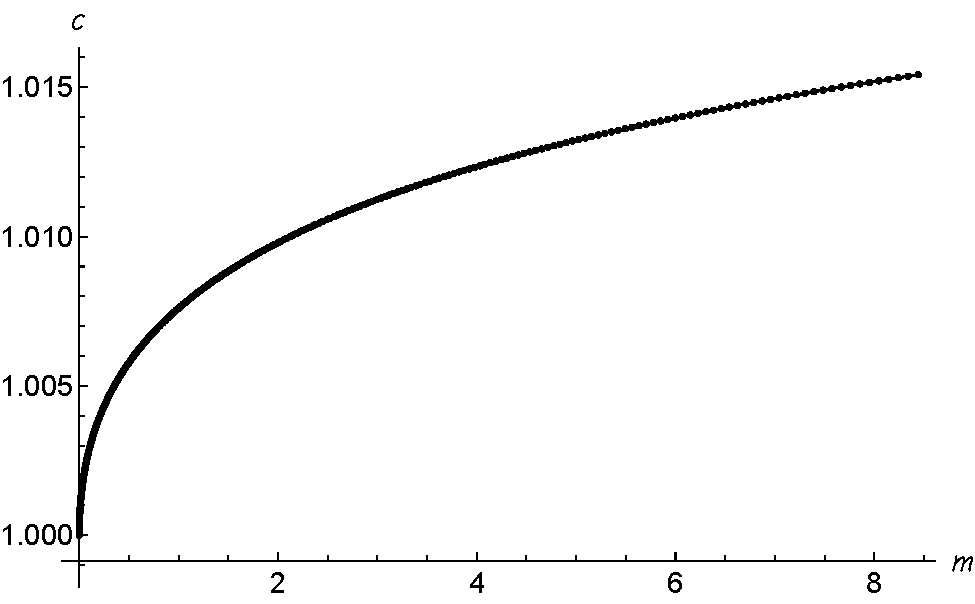
\includegraphics{\econtexRoot/\FigDirApndx/PFGICHoldsFHWCFailsRICFails}}
\caption{Nondegenerate Consumption Function with \cancel{FHWC} and \cancel{RIC}}
\label{fig:PFGICHoldsFHWCFailsRICFails}
\end{figure}

\begin{comment}
We can rewrite the expression for $\mathbb{C}$ from \eqref{PDVc} as:
\begin{eqnarray*}
   \mathbb{C}_{t-n}^{t} & = &  \left(\frac{\PatPGro^{-n}-\PatPGro^{-n}\PatR^{n+1}}{1-\PatR}\right)
\\ & = &  \left(\frac{\PatPGro^{-n}-\PatR\PGro^{n}/\Rfree^{n}}{1-\PatR}\right)
\\ & = &  \left(\frac{(\PGro/\Pat)^{n}-\PatR(\PGro/\Rfree)^{n}}{1-\PatR}\right)
\\ & = &  (\PGro/\Rfree)^{n}\left(\frac{(\Rfree/\Pat)^{n}-\PatR}{1-\PatR}\right)
\\ \Rnorm^{n}\mathbb{C}_{t-n}^{t}  & = &  \left(\frac{(\Rfree/\Pat)^{n}-\PatR}{1-\PatR}\right)
\end{eqnarray*}
but \cancel{RIC} implies that $\Pat > \Rfree$ so
\begin{eqnarray*}
\lim_{n \rightarrow \infty} \Rnorm^{n}\mathbb{C}_{t-n}^{t}  & = &  \left(\frac{-\PatR}{1-\PatR}\right)
\end{eqnarray*}
which means that in the limit
\begin{eqnarray}
\lim_{n \rightarrow \infty} \Rnorm^{n}\bRat_{\#}^{n} & = &  \left(\frac{-\PatR}{1-\PatR}\right) - \Rnorm^{n}\left(\frac{1-\Rnorm^{-1}\Rnorm^{-n}}{1-\Rnorm^{-1}}\right) %\label{eq:bPoundLim}
\\ & = & \left(\frac{-\PatR}{1-\PatR} + \frac{-\Rnorm^{-1}}{1-\Rnorm^{-1}}\right) - \left(\frac{\Rnorm^{n}}{1-\Rnorm^{-1}}\right)
\end{eqnarray}
so we can solve for the limiting $n$ as a function of $\bRat$ via
\begin{eqnarray}
  \bRat + \left(\frac{1}{1-\Rnorm^{-1}}\right) & = & \Rnorm^{-\hat{n}}\left(\frac{-\PatR}{1-\PatR} + \frac{-\Rnorm^{-1}}{1-\Rnorm^{-1}}\right)
\\ \log \left(\bRat + \left(\frac{1}{1-\Rnorm^{-1}}\right)\right) & = & -\hat{n} \log \Rnorm + \log \left(\frac{-\PatR}{1-\PatR} + \frac{-\Rnorm^{-1}}{1-\Rnorm^{-1}}\right)
\\ \frac{\log \left(\frac{-\PatR}{1-\PatR} + \frac{-\Rnorm^{-1}}{1-\Rnorm^{-1}}\right)-\log \left(\bRat + \left(\frac{1}{1-\Rnorm^{-1}}\right)\right)}{\log \Rnorm } & = & \hat{n}
\end{eqnarray}
which defines $\hat{\nFunc}(\bRat)$ which yields an approximation to the
value of $n$ associated with a given $\bRat$.

We can directly compute
\begin{eqnarray}
  \nabla & = & \bRat - \bRat_{\#}^{\hat{n}}
\end{eqnarray}
and can obtain a better appxoimation to the correct $n$ from
\begin{eqnarray}
  \hat{\hat{n}} & = &
\end{eqnarray}

We can obtain a more exact approximation to the correct ${n}$ by defining
\begin{eqnarray}
\nabla(n) \equiv   \lim_{n \rightarrow \infty}\Rnorm^{n}\mathbb{C}_{t-n}^{t}-\Rnorm^{n}\mathbb{C}_{t-n}^{t} & = &  \left(\frac{\PatR^{-n}}{1-\PatR}\right).
\end{eqnarray}
from which we can obtain the difference between the approximate and the exact $\mathbb{C}_{t-n}^{t}$ as $\Rnorm^{-n}\nabla(n)$ and


For this $n$ and
$\bRat$ we can obtain the corresponding
$\cRat=\PatPGro^{-\nFunc(\bRat)}$.  Note, however, that this is {\it not}
the level of $\cRat$ directly associated with $\bRat$ on the true
consumption function, because we used only a limiting approximation to
the correct $n$ rather than the correct $n$.

Our strategy, in this case, is

The limiting difference can be obtained by realizing that
\begin{eqnarray}
\nabla(n) \equiv   \lim_{n \rightarrow \infty}\Rnorm^{n}\mathbb{C}_{t-n}^{t}-\Rnorm^{n}\mathbb{C}_{t-n}^{t} & = &  \left(\frac{\PatR^{-n}}{1-\PatR}\right).
\end{eqnarray}
and so

\end{comment}

We can summarize as follows.  Given that the PF-GIC holds, the
interesting question is whether the FHWC holds.  If so, the
RIC automatically holds, and the solution limits
into the solution to the unconstrained problem as $\mRat \uparrow
\infty$.  But even if the FHWC fails, the problem has a
well-defined solution, whether or not the RIC holds.

%\end{verbatimwrite}\documentclass[../BufferStockTheory.tex]{subfiles}
\input{./econtexRoot} % Switch root to subdirectory 

\provideboolean{Metin}\setboolean{Metin}{true}\newcommand{\Metin}[2]{\ifthenelse{\boolean{Metin}}{\marginpar{\large Metin}\{{#1}\} $\rightarrow$ \{{#2}\}}{#2}}% PrivateMsg: Comments by Metin Uyanik

\begin{document}
\newcommand{\FigDirApndx}{Code/Mathematica/Results/BufferStockTheory/Figures}

%\begin{verbatimwrite}{\ApndxDir/ApndxSolnMethEndogGpts.tex}
\section{Perfect Foresight Liquidity Constrained Solution}\label{sec:ApndxLiqConstr}
%{\it Note: There is an inconsistency between the files ApndxLiqConstr.tex and ApndxLiqConstrStandAlone.tex files in the beginning of the first paragraph below. I accept ApndxLiqConstr.tex as valid and replace the first paragraph in this StandAlone version with the one in the output file. This seems counterintuitive since ApndxLiqConstr.tex is output of ApndxLiqConstrStandAlone.tex but the paragraph in the ApndxLiqConstr.tex file sounds better.} % MetinComment % PrivateMsg

  This appendix taxonomizes the characteristics of the limiting
  consumption function $\mathring{\cFunc}(\mRat)$ under perfect
  foresight in the presence of a liquidity constraint requiring $\bRat
  \geq 0$ under various conditions.  Results are summarized in
  table~\ref{table:LiqConstrScenarios}.

\input{\econtexRoot/\TableDir/LiqConstrScenarios.tex}

\subsection{If PF-GIC Fails}

A consumer is `growth patient' if the perfect foresight growth
impatience condition fails (\cancel{PF-GIC}, $1 < \Pat/\PGro$).  Under
\cancel{PF-GIC} the constraint does not bind at the lowest feasible value of $\mRat_{t}=1$ because
$1 < (\Rfree\Discount)^{1/\CRRA}/\PGro$ implies that spending
everything today (setting $\cRat_{t}=\mRat_{t}=1$) produces lower
marginal utility than is obtainable by reallocating a marginal unit of
resources to the next period at return $\Rfree$:\footnote{The point at
  which the constraint would bind (if that point could be attained) is
  the $\mRat=\cRat$ for which $\util^{\prime}(\cRat_{\#}) = \Rfree
  \Discount \util^{\prime}(\PGro)$ which is $\cRat_{\#} =
  \PGro/(\Rfree \Discount)^{1/\CRRA}$ and the consumption function
  will be defined by
  $\mathring{\cFunc}(\mRat)=\min[\mRat,\cRat_{\#}+(\mRat-\cRat_{\#})\MinMPC
  ]$.}
\begin{eqnarray}
1 & < & (\Rfree \Discount)^{1/\CRRA}\PGro^{-1}   \label{eq:EulerPFGICFails}
\\ 1 & < & \Rfree \Discount \PGro^{-\CRRA}
\\  \util^{\prime}(1) & < & \Rfree \Discount \util^{\prime}(\PGro)   \label{eq:EulerPFGICFailsEnd}.
\end{eqnarray}

Similar logic shows that under these circumstances the constraint will
never bind for a constrained consumer with a finite horizon of $n$
periods, so such a consumer's consumption function will be the same as for the
unconstrained case examined in the main text.

If the RIC fails ($1 < \PatR$) while the finite human wealth condition
holds, the limiting value of this consumption function as $n \uparrow
\infty$ is the degenerate function
\begin{eqnarray}
  \mathring{\cFunc}_{T-n}(\mRat) & = & 0 (\bRat_{t}+\hRat).
\end{eqnarray}

If the RIC fails and the FHWC fails, human wealth limits to $\hRat =
\infty$ so the consumption function limits to either
$\mathring{\cFunc}_{T-n}(\mRat) = 0$ or
$\mathring{\cFunc}_{T-n}(\mRat) = \infty$ depending on the relative
speeds with which the MPC approaches zero and human wealth approaches
$\infty$.\footnote{The knife-edge case is where $\Pat = \PGro$, in
  which case the two quantites counterbalance and the limiting
  function is $\mathring{\cFunc}(\mRat)=\min[\mRat,1]$.}

Thus, the requirement that the consumption function be nondegenerate
implies that for a consumer satisfying \cancel{PF-GIC} we must impose
the RIC (and the FHWC can be shown to be a consequence of \cancel{PF-GIC} and RIC).  In
this case, the consumer's optimal behavior is easy to describe.  We
can calculate the point at which the unconstrained consumer would
choose $\cRat = \mRat$ from \eqref{eq:cFuncPFUnc}:
\begin{eqnarray}
  \mRat_{\#} & = & (\mRat_{\#}-1+\hRat)\MinMPC
\\ \mRat_{\#}(1-\MinMPC) & = & (\hRat - 1)\MinMPC
\\ \mRat_{\#} & = & (\hRat - 1)\left(\frac{\MinMPC}{1-\MinMPC}\right)
\end{eqnarray}
which (under these assumptions) satisfies $0 < \mRat_{\#} < 1$.\footnote{Note that $0 < \mRat_{\#}$ is implied by RIC and $ \mRat_{\#}<1$ is implied by \mbox{\cancel{PF-GIC}}.}  For
$\mRat < \mRat_{\#}$ the unconstrained consumer would choose to
consume more than $\mRat$; for such $\mRat$, the constrained consumer
is obliged to choose $\mathring{\cFunc}(\mRat) = \mRat$.\footnote{As an
  illustration, consider a consumer for whom $\Pat = 1$, $\Rfree
  =1.01$ and $\PGro = 0.99$.  This consumer will save the amount
  necessary to ensure that growth in market wealth exactly offsets the
  decline in human wealth represented by $\PGro < 1$; total wealth
  (and therefore total consumption) will remain constant, even as
  market wealth and human wealth trend in opposite directions.}  For
any $\mRat > \mRat_{\#}$ the constraint will never bind and the
consumer will choose to spend the same amount as the unconstrained
consumer, $\bar{\cFunc}(\mRat)$.


\subsection{If PF-GIC Holds}

Imposition of the PF-GIC reverses the inequality in
\eqref{eq:EulerPFGICFails}-\eqref{eq:EulerPFGICFailsEnd}, and thus
reverses the conclusion: A consumer who starts with $\mRat_{t}=1$ will
desire to consume more than 1.  Such a consumer will be constrained,
not only in period $t$, but perpetually thereafter.

Now define $\bRat_{\#}^{n}$ as the $\bRat_{t}$ such that
an unconstrained consumer holding $\bRat_{t}=\bRat_{\#}^{n}$ would behave so as to arrive in period $t+n$ with $\bRat_{t+n}=0$ (with $\bRat_{\#}^{0}$ trivially equal to 0); for example, a consumer with $\bRat_{t-1}=\bRat_{\#}^{1}$ was on the `cusp' of being constrained in period
$t-1$: Had $b_{t-1}$ been infinitesimally smaller, the constraint
would have been binding (because the consumer would have desired, but
been unable, to enter period $t$ with negative, not zero, $b$).  Given
the PF-GIC, the constraint certainly binds in period $t$ (and
thereafter) with resources of
$\mRat_{t}=\mRat_{\#}^{0}=1+\bRat_{\#}^{0}=1$: The consumer cannot
spend more (because constrained), and will not choose to spend less
(because impatient), than $c_{t}=\cRat_{\#}^{0}=1$.

We can construct the entire `prehistory' of this consumer leading up to $t$ as follows.
Maintaining the assumption that the constraint has never bound in the past,
$\cRat$ must have been growing according to $\PatPGro$, so consumption $n$ periods in the past must have been
\begin{eqnarray}
  \cRat_{\#}^{n} & = & \PatPGro^{-n} \cRat_{t} = \PatPGro^{-n}. \label{eq:cPreHist}
\end{eqnarray}

The PDV of consumption from $t-n$ until $t$ can thus be computed as
\begin{eqnarray}
   \mathbb{C}_{t-n}^{t} & = & \cRat_{t-n}(1+\Pat/\Rfree+ ... + (\Pat/\Rfree)^{n}) \notag
% \\   \mathbb{C}_{t-n}^{t} & = & \cRat_{t-n}(1+\PatPGro/\Rnorm+ ... + (\PatPGro/\Rnorm)^{n}) \notag
\\ & = & \cRat_{\#}^{n}(1+\PatR+ ... + \PatR^{n}) \notag
\\ & = & \PatPGro^{-n}\left(\frac{1-\PatR^{n+1}}{1-\PatR}\right) \label{PDVc}
\end{eqnarray}
and note that the consumer's human wealth between $t-n$ and $t$ (the relevant
time horizon, because from $t$ onward the consumer will be constrained
and unable to access post-$t$ income) is
\begin{eqnarray}
  \hRat_{\#}^{n} & = & 1+...+\Rnorm^{-n}
\end{eqnarray}
while the intertemporal budget constraint says
\begin{eqnarray*}
  \mathbb{C}_{t-n}^{t} & = & \bRat_{\#}^{n}+\hRat_{\#}^{n}
\end{eqnarray*}
from which we can solve for the $\bRat_{\#}^{n}$ such that
the consumer with $\bRat_{t-n} = \bRat_{\#}^{n}$ would
unconstrainedly plan (in period $t-n$) to arrive in period $t$ with
$\bRat_{t}=0$:
\begin{eqnarray}
\bRat_{\#}^{n} & =&  \mathbb{C}_{t-n}^{t} - \overbrace{\left(\frac{1-\Rnorm^{-(n+1)}}{1-\Rnorm^{-1}}\right)}^{\hRat_{\#}^{n}} \label{eq:bPound}.
\end{eqnarray}

Defining $\mRat_{\#}^{n}=\bRat_{\#}^{n}+1$, consider the function
$\mathring{\cFunc}(\mRat)$ defined by linearly connecting the points
$\{\mRat_{\#}^{n},\cRat_{\#}^{n}\}$ for integer values of $n \geq 0$
(and setting $\mathring{\cFunc}(\mRat)=\mRat$ for $\mRat<1$).  This
function will return, for any value of $\mRat$, the optimal value of
$\cRat$ for a liquidity constrained consumer with an infinite horizon.
The function is piecewise linear with `kink points' where the slope
discretely changes, because for infinitesimal $\epsilon$ the MPC of a
consumer with assets $\mRat=\mRat_{\#}^{n}-\epsilon$ is discretely
higher than for a consumer with assets $\mRat=\mRat_{\#}^{n}+\epsilon$
because the latter consumer will spread a marginal dollar over more
periods before exhausting it.

In order for a unique consumption function to be defined by this
sequence \eqref{eq:bPound} for the entire domain of positive real
values of $b$, we need $\bRat_{\#}^{n}$ to become arbitrarily large with
$n$.  That is, we need
\begin{eqnarray}
  \lim_{n \rightarrow \infty} \bRat_{\#}^{n} = \infty. \label{eq:bToInfty}
\end{eqnarray}

\subsubsection{If FHWC Holds}
The FHWC requires $\Rnorm^{-1} < 1$, in which case the second term in \eqref{eq:bPound} limits to a constant as $n \uparrow \infty$, and \eqref{eq:bToInfty} reduces to a requirement that
\begin{eqnarray*}
  \lim_{n \rightarrow \infty} \left(\frac{\PatPGro^{-n}-(\PatR/\PatPGro)^{n}\PatR}{1-\PatR}\right) & = & \infty
\\  \lim_{n \rightarrow \infty} \left(\frac{\PatPGro^{-n}-\Rnorm^{-n}\PatR}{1-\PatR}\right) & = & \infty
\\  \lim_{n \rightarrow \infty} \left(\frac{\PatPGro^{-n}}{1-\PatR}\right) & = & \infty.
\end{eqnarray*}
Given the PF-GIC $\PatPGro^{-1}>1$, this will hold iff the RIC holds, $\PatR < 1$.  But given that the FHWC
$\Rfree > \PGro$ holds, the PF-GIC is stronger (harder to satisfy) than the RIC; thus, FHWC
and the PF-GIC together imply the RIC, and so a well-defined
solution exists.  Furthermore, in the limit as $n$ approaches
infinity, the difference between the limiting constrained consumption
function and the unconstrained consumption function becomes
vanishingly small, because as the date at which the constraint binds
becomes arbitrarily distant, the effect of that constraint on current
behavior shrinks to nothing.  That is,
\begin{eqnarray}
\lim_{m \rightarrow \infty}\mathring{\cFunc}(m) - \bar{\cFunc}(m) = 0.
\end{eqnarray}

% Finally, the main text shows that the PF-GIC is a stronger condition than the PF-FVR; that is, PF-GIC $\Rightarrow$ PF-FVR.

\subsubsection{If FHWC Fails}
If the FHWC fails, matters are a bit more complex.
\begin{comment}
As noted in the main text, the Finite Value Requirement for such a consumer
requires $\PatPGro < (\Rfree/\PGro)^{1/\CRRA}$,\footnote{A
  unique well-defined nondegenerate limiting consumption function can
  actually exist even if a nondegenerate value function does not.  But
  the parametric combinations required for this are somewhat peculiar
  (including both $\Rfree < 1$ and $\PGro < 1$); but we restrict our attention
  to the more useful and plausible cases with finite value.} which is stronger (holds
in strictly fewer circumstances) than the PF-GIC condition $\PatPGro < 1$.
Thus, the PF-GIC is an implication of \cancel{FHWC}.
\end{comment}
Given failure of FHWC, \eqref{eq:bToInfty} requires

\begin{eqnarray}
%  \lim_{n \rightarrow \infty} \left(\frac{\PatPGro^{-n}-\Rnorm^{-n}\PatR}{1-\PatR}\right) + \left(\frac{1-\Rnorm^{-(n+1)}}{\Rnorm^{-1}-1}\right) & = & \infty \\
  \lim_{n \rightarrow \infty} \left(\frac{\Rnorm^{-n}\PatR-\PatPGro^{-n}}{\PatR-1}\right) + \left(\frac{1-\Rnorm^{-(n+1)}}{\Rnorm^{-1}-1}\right) & = & \infty \notag
\\   \lim_{n \rightarrow \infty} \left(\frac{\PatR}{\PatR-1}-\frac{\Rnorm^{-1}}{\Rnorm^{-1}-1}\right)\Rnorm^{-n}-\left(\frac{\PatPGro^{-n}}{\PatR-1}\right) & = & \infty \notag
\\   \lim_{n \rightarrow \infty} \left(\frac{\PatR(\Rnorm^{-1}-1)}{(\Rnorm^{-1}-1)(\PatR-1)}-\frac{\Rnorm^{-1}(\PatR-1)}{(\Rnorm^{-1}-1)(\PatR-1)}\right)\Rnorm^{-n}-\left(\frac{\PatPGro^{-n}}{\PatR-1}\right) & = & \infty. \label{eq:FHWCfails}
\end{eqnarray}

{\bf If RIC Holds}.  When the RIC holds, rearranging \eqref{eq:FHWCfails} gives
\begin{eqnarray*}
  \lim_{n \rightarrow \infty} \left(\frac{\PatPGro^{-n}}{1-\PatR}\right)-\Rnorm^{-n}\left(\frac{\PatR}{1-\PatR}+\frac{\Rnorm^{-1}}{\Rnorm^{-1}-1}\right) & = & \infty
\end{eqnarray*}
and for this to be true we need
\begin{eqnarray*}
  \PatPGro^{-1} & > & \Rnorm^{-1}
\\ \PGro/\Pat & > & \PGro/\Rfree
\\ 1 & > & \Pat/\Rfree
\end{eqnarray*}
which is merely the RIC again.  So the problem has a solution if the RIC holds.  Indeed,
we can even calculate the limiting MPC from
\begin{eqnarray}
  \lim_{n \rightarrow \infty} \MPC^{n}_{\#} & = & \lim_{n \rightarrow \infty} \left(\frac{\cRat_{\#}^{n}}{\bRat_{\#}^{n}}\right)
\end{eqnarray}
which with a few lines of algebra
\begin{comment}
Calculate the limit of
\begin{eqnarray}
\left(\frac{\PatPGro^{-n}}{\PatPGro^{-n}/(1-\PatR) - (1-\Rnorm^{-1}\Rnorm^{-n})/(1-\Rnorm^{-1})}\right) & = & \left(\frac{1}{1/(1-\PatR) + \Rnorm^{-n}\Rnorm^{-1}/(1-\Rnorm^{-1})}\right)
\end{eqnarray}
\end{comment}
can be shown to asymptote to the MPC in the perfect foresight model:\footnote{For an example of this configuration of parameters, see the notebook \texttt{doApndxLiqConstr.nb} in the software archive.}
\begin{eqnarray}
  \lim_{m \rightarrow \infty} \mathring{\pmb{\MPC}}(\mRat) & = & 1-\PatR.
\end{eqnarray}

{\bf If RIC Fails}.  Consider now the \cancel{RIC} case, $\PatR > 1$.  In this case the constant multiplying
$\Rnorm^{-n}$ in \eqref{eq:FHWCfails} will be positive if
\begin{eqnarray*}
  \PatR \Rnorm^{-1} - \PatR & > &  \Rnorm^{-1}\PatR-\Rnorm^{-1}
\\ \Rnorm^{-1} & > & \PatR
\\ \PGro & > & \Pat
\end{eqnarray*}
which is merely the PF-GIC which we are maintaining.  So the first term's limit is $+\infty$.  The
combined limit will be $+\infty$ if the term involving $\Rnorm^{-n}$
goes to $+\infty$ faster than the term involving $-\PatPGro^{-n}$ goes to
$-\infty$; that is, if
\begin{eqnarray*}
  \Rnorm^{-1} & > & \PatPGro^{-1}
\\ \PGro/\Rfree & > & \PGro/\Pat
\\ \Pat/\Rfree & > & 1
\end{eqnarray*}
which merely confirms the starting assumption that the RIC fails.
Thus, surprisingly, the problem has a well defined solution with
infinite human wealth if the RIC fails.  It remains true that \cancel{RIC}
implies a limiting MPC of zero,
\begin{eqnarray}
  \lim_{\mRat \rightarrow \infty} \mathring{\pmb{\MPC}}(\mRat)  & = & 0,
\end{eqnarray}
but that limit is approached gradually, starting from a positive
value, and consequently the consumption function is {\it not} the
degenerate $\mathring{\cFunc}(\mRat)=0$.  (Figure~\ref{fig:PFGICHoldsFHWCFailsRICFails} presents an example for $\CRRA=2$, $\Rfree=0.98$, $\Discount = 0.99$, $\PGro = 1.0$).

\begin{figure}
\centerline{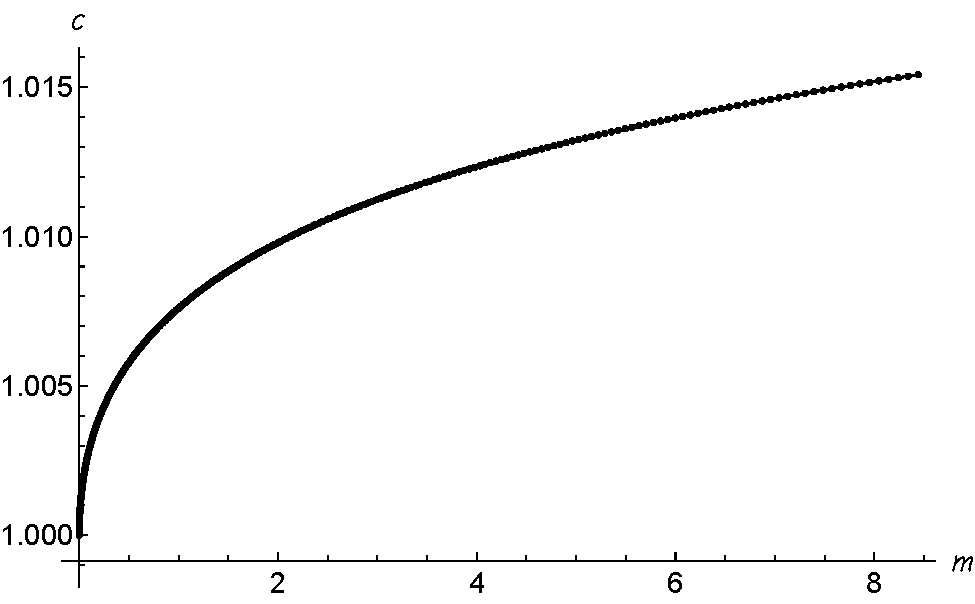
\includegraphics{\econtexRoot/\FigDirApndx/PFGICHoldsFHWCFailsRICFails}}
\caption{Nondegenerate Consumption Function with \cancel{FHWC} and \cancel{RIC}}
\label{fig:PFGICHoldsFHWCFailsRICFails}
\end{figure}

\begin{comment}
We can rewrite the expression for $\mathbb{C}$ from \eqref{PDVc} as:
\begin{eqnarray*}
   \mathbb{C}_{t-n}^{t} & = &  \left(\frac{\PatPGro^{-n}-\PatPGro^{-n}\PatR^{n+1}}{1-\PatR}\right)
\\ & = &  \left(\frac{\PatPGro^{-n}-\PatR\PGro^{n}/\Rfree^{n}}{1-\PatR}\right)
\\ & = &  \left(\frac{(\PGro/\Pat)^{n}-\PatR(\PGro/\Rfree)^{n}}{1-\PatR}\right)
\\ & = &  (\PGro/\Rfree)^{n}\left(\frac{(\Rfree/\Pat)^{n}-\PatR}{1-\PatR}\right)
\\ \Rnorm^{n}\mathbb{C}_{t-n}^{t}  & = &  \left(\frac{(\Rfree/\Pat)^{n}-\PatR}{1-\PatR}\right)
\end{eqnarray*}
but \cancel{RIC} implies that $\Pat > \Rfree$ so
\begin{eqnarray*}
\lim_{n \rightarrow \infty} \Rnorm^{n}\mathbb{C}_{t-n}^{t}  & = &  \left(\frac{-\PatR}{1-\PatR}\right)
\end{eqnarray*}
which means that in the limit
\begin{eqnarray}
\lim_{n \rightarrow \infty} \Rnorm^{n}\bRat_{\#}^{n} & = &  \left(\frac{-\PatR}{1-\PatR}\right) - \Rnorm^{n}\left(\frac{1-\Rnorm^{-1}\Rnorm^{-n}}{1-\Rnorm^{-1}}\right) %\label{eq:bPoundLim}
\\ & = & \left(\frac{-\PatR}{1-\PatR} + \frac{-\Rnorm^{-1}}{1-\Rnorm^{-1}}\right) - \left(\frac{\Rnorm^{n}}{1-\Rnorm^{-1}}\right)
\end{eqnarray}
so we can solve for the limiting $n$ as a function of $\bRat$ via
\begin{eqnarray}
  \bRat + \left(\frac{1}{1-\Rnorm^{-1}}\right) & = & \Rnorm^{-\hat{n}}\left(\frac{-\PatR}{1-\PatR} + \frac{-\Rnorm^{-1}}{1-\Rnorm^{-1}}\right)
\\ \log \left(\bRat + \left(\frac{1}{1-\Rnorm^{-1}}\right)\right) & = & -\hat{n} \log \Rnorm + \log \left(\frac{-\PatR}{1-\PatR} + \frac{-\Rnorm^{-1}}{1-\Rnorm^{-1}}\right)
\\ \frac{\log \left(\frac{-\PatR}{1-\PatR} + \frac{-\Rnorm^{-1}}{1-\Rnorm^{-1}}\right)-\log \left(\bRat + \left(\frac{1}{1-\Rnorm^{-1}}\right)\right)}{\log \Rnorm } & = & \hat{n}
\end{eqnarray}
which defines $\hat{\nFunc}(\bRat)$ which yields an approximation to the
value of $n$ associated with a given $\bRat$.

We can directly compute
\begin{eqnarray}
  \nabla & = & \bRat - \bRat_{\#}^{\hat{n}}
\end{eqnarray}
and can obtain a better appxoimation to the correct $n$ from
\begin{eqnarray}
  \hat{\hat{n}} & = &
\end{eqnarray}

We can obtain a more exact approximation to the correct ${n}$ by defining
\begin{eqnarray}
\nabla(n) \equiv   \lim_{n \rightarrow \infty}\Rnorm^{n}\mathbb{C}_{t-n}^{t}-\Rnorm^{n}\mathbb{C}_{t-n}^{t} & = &  \left(\frac{\PatR^{-n}}{1-\PatR}\right).
\end{eqnarray}
from which we can obtain the difference between the approximate and the exact $\mathbb{C}_{t-n}^{t}$ as $\Rnorm^{-n}\nabla(n)$ and


For this $n$ and
$\bRat$ we can obtain the corresponding
$\cRat=\PatPGro^{-\nFunc(\bRat)}$.  Note, however, that this is {\it not}
the level of $\cRat$ directly associated with $\bRat$ on the true
consumption function, because we used only a limiting approximation to
the correct $n$ rather than the correct $n$.

Our strategy, in this case, is

The limiting difference can be obtained by realizing that
\begin{eqnarray}
\nabla(n) \equiv   \lim_{n \rightarrow \infty}\Rnorm^{n}\mathbb{C}_{t-n}^{t}-\Rnorm^{n}\mathbb{C}_{t-n}^{t} & = &  \left(\frac{\PatR^{-n}}{1-\PatR}\right).
\end{eqnarray}
and so

\end{comment}

We can summarize as follows.  Given that the PF-GIC holds, the
interesting question is whether the FHWC holds.  If so, the
RIC automatically holds, and the solution limits
into the solution to the unconstrained problem as $\mRat \uparrow
\infty$.  But even if the FHWC fails, the problem has a
well-defined solution, whether or not the RIC holds.

%\end{verbatimwrite}\input {\ApndxDir/ApndxLiqConstr.tex}

\end{document}


\end{document}


\end{document}


\end{document}
